%%%%%%%%%%%%%%%%%%%%%%%%%%%%%%%%%%%%%%%%%%%%%%%
%
% Template for Master degrees
% DISI - Dipartimento di Ingegneria e Scienza dell’Informazione
% DISI - Department of Information Engineering and Computer Science
%
% update 2020-08-30
%
% To generate pdf 
% pdflatex __filename__.tex
% bibtex __file_name__.aux
% pdflatex __file_name__.tex
% pdflatex __file_name__.tex
%
%%%%%%%%%%%%%%%%%%%%%%%%%%%%%%%%%%%%%%%%%%%%%%%

% 2 side format
% \documentclass[epsfig,a4paper,11pt,titlepage,twoside,openany]{book}
\documentclass[a4paper,11pt,titlepage,twoside,openany]{book}
\usepackage{epsfig}
\usepackage{plain}
\usepackage{setspace}
\usepackage[paperheight=29.7cm,paperwidth=21cm,outer=1.5cm,inner=2.5cm,top=2cm,bottom=2cm]{geometry} % layout setting
\usepackage{titlesec} % custom setup title of chanpter
% \usepackage{newtxtext,newtxmath} % times new roman
\usepackage{hyperref}

% ATTENTION --- Added by me
\usepackage{multirow, multicol, array, enumitem, amsmath, pdfpages}

% --------------------------

% support for accented letters
%
%\usepackage[latin1]{inputenc} % Windows;
\usepackage[utf8x]{inputenc} % Linux (unicode package is required);
%\usepackage[applemac]{inputenc} % Mac.

\singlespacing

% italian language
%\usepackage[italian]{babel}

\begin{document}

  % no page number
  \pagenumbering{gobble} 
  \pagestyle{plain}

\thispagestyle{empty}

\begin{center}
  \begin{figure}[h!]
    \centerline{
\psfig{file=marchio_unitrento_colore_it_202002.eps,width=0.6\textwidth}}
  \end{figure}

  \vspace{2 cm} 

  \LARGE{Department of Information Engineering and Computer Science\\}

  \vspace{1 cm} 
  \Large{Master's Degree in\\
    Computer Science
    % Computer, Communication and Electronic Engineering
    % Information and Communications Engineering
    % Information and Business Organization Engineering
    % Electornics and Telecommunications Engineerign
  }

  \vspace{2 cm} 
  \Large\textsc{Final Dissertation\\} 
  \vspace{1 cm} 
  % to define
  \Huge\textsc{Sustainable Digital Education Technologies in Universities: a multi-dimensional framework}
  % \Large{\it{Sub-title (optional)}}


  \vspace{2 cm} 
  \begin{tabular*}{\textwidth}{ c @{\extracolsep{\fill}} c }
  \Large{Supervisor} & \Large{Student}\\
  \Large{Dr Lorenzo Angeli}& \Large{Sebastiano Cassol}\\
  \end{tabular*}

  \vspace{2 cm} 

  \Large{Academic year 2023/2024}
  
\end{center}



  \cleardoublepage
 
% Thanks/ Acknowledgements section
  \thispagestyle{empty}

\begin{center}
  {\bf \Huge Acknowledgements}
\end{center}

\vspace{4cm}


\emph{
Firstly, I want to express my deepest gratitude to Dr Lorenzo Angeli, who has guided and assisted me during the writing of this thesis.
}

\bigskip

\emph{
Thanks to my parents and my family, who have supported and accompanied me on this journey.
}

\bigskip

\emph{
Thanks to my friends for all the laughter and wonderful moments we shared together.
}

\bigskip

\emph{
Thanks to my dogs, both those still by my side and those who are not, for keeping me company through countless nights in front of the screen.
}

\bigskip

\emph{
Finally, a heartfelt thanks to my girlfriend, Anastasia, for her endless patience, for always standing by my side, for being my number one supporter.
}
  \clearpage
  \pagestyle{plain} % no heading, footer with centered page number

  
  % page number with Arabic format
  \mainmatter

%% Note
%% Length: approximately 70 pages.
%% These 70 pages include:
%%   table of contents
%%   abstract
%%   chapters
%% Exclude:
%%   title page
%%   acknowledgments
%%   attachments

    % index
    \tableofcontents
    \clearpage
          
    % group to define space between chapters
    \begingroup
      % no page break between chapters
      % override clear page commands
      \renewcommand{\cleardoublepage}{} 
      \renewcommand{\clearpage}{} 
      % override format of title chapter
      % from
      %   Chapter X
      %   Title
      % to
      %   X   Title
      
      \titleformat{\chapter}
        {\normalfont\Huge\bfseries}{\thechapter}{1em}{}
        
      \titlespacing*{\chapter}{0pt}{0.59in}{0.02in}
      \titlespacing*{\section}{0pt}{0.20in}{0.02in}
      \titlespacing*{\subsection}{0pt}{0.10in}{0.02in}
      
      % summary / abstract
      \chapter*{Abstract} % no number
\label{abtract}

\addcontentsline{toc}{chapter}{Abstract} % add to index

\bigskip

The rapid adoption of Digital Education Technologies (DETs) has transformed higher education, improving accessibility, collaboration, and administrative efficiency. However, universities often lack structured sustainability assessment frameworks, selecting DETs that lead to vendor lock-in, data privacy concerns, environmental impact, and limited institutional control over digital infrastructures. While cloud-based solutions offer convenience and scalability, they may compromise long-term sustainability and autonomy.

This thesis develops a multi-dimensional sustainability framework to evaluate DETs across technical, economic, social, pedagogical, and environmental dimensions. The framework introduces a structured methodology and a traffic-light scoring system to guide decision-makers in selecting sustainable and ethical digital solutions. The assessment is designed to balance trade-offs between cost efficiency, pedagogical value, institutional control, and environmental impact, ensuring a holistic evaluation process.

To validate the framework, it is applied to Overleaf, a collaborative LaTeX platform, comparing its Community Edition, Server Pro, and cloud-based versions. The results highlight key sustainability trade-offs: while the cloud version excels in economic and technical efficiency, it raises concerns about data privacy and environmental impact. Conversely, self-hosted versions provide greater institutional control and autonomy, but require higher technical expertise and resource investment. The assessment also reveals that pedagogical quality remains unaffected by deployment choice, reinforcing the importance of other sustainability dimensions in the selection process.

A critical discussion on scoring limitations and the challenge of multi-dimensionality underscores the need for future refinements, including weighted indicators to ensure a balanced evaluation. The research concludes that if DETs fail entirely in one sustainability dimension, their adoption should be reconsidered, emphasizing the interdependence of sustainability factors.

By providing a structured and adaptable evaluation framework, this study contributes to sustainable digital transformation in higher education, equipping universities with a transparent decision-making tool to align technology adoption with institutional, ethical, and long-term sustainability goals.





      \newpage
      \ % The empty page
      \newpage

%% Note
%% The first chapter of the final thesis must contain a summary of a 
%% maximum length of 3 pages, introducing the context and motivations,
%% resuming the problem faced by the student, the techniques used for the
%% investigation and the reached outcomes.
%% If the final thesis is developed in collaboration with other students,
%% the personal contribution of the student has to be underlined. 
      
      %%%%%%%%%%%%%%%%%%%%%%%%%%%%%%%%
      % chapters
      %
      % \input or \include
      %
      \chapter{Introduction}
\label{cha:1_intro}
The rapid advancement of digital education technologies (DETs) has significantly transformed higher education, reshaping the learning experience and the management of academic activities within the institutions \cite{haleem_understanding_2022}\cite{lacka_examining_2021}. DETs, which encompass a broad range of software and hardware technologies, have played a central role in improving educational accessibility and addressing global challenges in education \cite{schuetze_digitalization_2024}, representing a powerful instrument to achieve the United Nations Sustainable Development Goal 4 for Quality Education.

However, the increasing digitalization of universities has raised many concerns about data privacy, economic dependencies, and institutional autonomy \cite{fiebig_heads_2023}\cite{komljenovic_rise_2021}. The growing reliance on solutions provided by Big Tech companies has intensified worries about the risk of lock-in and loss of data governance, creating a degree of uncertainty regarding the long-term sustainability of these digital infrastructures \cite{angeli_conceptualising_2022}. In addition, the energy consumption and environmental footprint of digital education platforms bring new challenges in aligning technological innovation with sustainability \cite{lago_framing_2015}.

This thesis aims to improve and facilitate the selection process of digital education technologies. To achieve this, it proposes a comprehensive framework that evaluates DETs across all aspects of sustainability, providing a clearer overall picture that highlights the critical strengths and weaknesses of each technology.

\section{Digitalization in Higher Education}
The phenomenon of digitalization, driven by rapid advancements in information and communication technologies (ICT), has led to the widespread adoption of digital education technologies. The integration of the first DETs, such as Learning Management Systems (LMS) and administrative tools, enabled institutions to digitalize content delivery, facilitate student engagement, online learning e administrative tasks \cite{lacka_examining_2021}. With the rise of internet and mobile computing, digital learning further evolved to incorporate new technologies, such as video conferencing tools, and increasingly relying on cloud-based infrastructures. The rapid shift forced by the pandemic exposed strength and weaknesses of digital education, highlighting its potential to improve accessibility while also revealing technical, economic, and social barriers for students and instructors \cite{schuetze_digitalization_2024}.

The outsourcing trend toward Big Tech cloud ecosystems, driven by financial and operational pressures, has allowed universities to quickly adapt to changing educational needs while benefiting of cost efficiency and technical expertise of industry leaders \cite{komljenovic_rise_2021}. However, this trend raised concerns about the outsourcing of university core services, making institutions ever more dependent on private corporations \cite{angeli_conceptualising_2022}. The reliance on cloud providers has also ethical and environmental implications. While many companies claim to limit their environmental impact, many data centers still rely on non-renewable energy, contributing to environmental pollution. Moreover, the continuous upgrading of DETs accelerates hardware obsolescence, contributing to e-waste production and resource depletion. In addition to the diminished control over their own environmental impact, institutions face also the loss of power over data governance, particularly regarding the collection and use of student data \cite{komljenovic_rise_2021}.

All these factors emphasize the need to adopt a critical approach to digitalization, ensuring that universities can make informed, sustainable, and ethical decisions when selecting their digital education technologies. Despite the potential benefits of DETs, the process of selecting technologies that align with institutional values remains a complex challenge.

% \section{The problem of DETs selection}

\section{Knowledge gaps}
Identified knowledge gaps in digital education technologies are as follows:
\begin{itemize}[noitemsep, topsep=4pt, parsep=0pt, partopsep=0pt]
\item While digital education technologies continue to be introduced in higher education institutions, there is still a lack on standardized processes and guidelines about how to select a sustainable DETs 
\item Even though some sustainability aspects are considered more than others in the actual DET selection processes, it is not clear which dimensions of sustainability are involved in the context of education technologies
\item Research literature on digital education does not focus on evaluating or enhancing sustainability of DET, instead it concentrates more on their impact in higher education
\end{itemize}

\section{Goals}
The main goal of this research is to develop a sustainability assessment framework for digital education technologies in universities. Specifically, the study aims to:
\begin{itemize}[noitemsep, topsep=4pt, parsep=0pt, partopsep=0pt]
\item Define the concept of sustainability in the context of DETs, by integrating the relevant dimension identified from research literature.
\item Provide a structured approach for universities that assists those responsible for selection to assess the sustainability of DETs, before the adoption.
\item Demonstrate and discuss its real-world applicability by applying the framework to a DET.
\end{itemize}
Based on the knowledge gaps and goals listed above, this thesis will attempt to answer the following questions:
\begin{center}
    \textit{\textbf{"How can higher education institutions evaluate the sustainability of digital education technologies?"}} \\
    \textit{\textbf{"How can universities facilitate and structure the DET selection process?"}}
\end{center}

% By achieving these goals, this research contributes to the ongoing discourse on sustainable digital education and offers practical guidelines for institutions seeking to adopt responsible digitalization strategies.

\section{Research methodology}
The methodology employed in this study follows a structured approach. First, the research literature was collected and reviewed to identify key dimensions for DETs. Then, the framework was developed based on the outcome of this review and was finally applied to a real-world case study. 
%on those dimensions, defining indicators and evaluation methods. Finally, the framework was applied to a real-world DET, Overleaf, to assess is sustainability and compliance with the defined indicators. 

\subsection{Research literature}
The literature was collected through various methods. First, the literature recommended by the supervisor was reviewed, covering topics related to sustainability frameworks, digital education technologies, and digitalization. From this initial set of sources, both cited and citing articles were examined to expand the collection. Finally, additional articles were retrieved through search engines and Google Scholar. The search queries included combinations of the following keywords: "education", "digital education", "digital education technology", "sustainability", "framework", "indicators", "energy consumption", "emissions", "metrics", "inclusion", "accessibility", "university", and "data center".

\subsection{Framework development}
The framework was developed based on the key sustainability dimensions identified in the literature review. These dimensions provided the foundation for defining relevant indicators, metrics, and evaluation methods to assess the sustainability of digital education technologies. 

First, the selected dimensions were analyzed to determine their applicability to DETs. Then, specific indicators were defined for each dimension, ensuring they were measurable and aligned with sustainability principles. Subsequently, evaluation methods were identified, drawing from established assessment techniques in sustainability and digital education research. In cases where no existing methods were suitable, new evaluation approaches and metrics were developed, as some aspects of sustainability in DETs remain under active research.

\subsection{Case study analysis}
To validate the proposed framework, it was applied to a real-world digital education technology: Overleaf, a collaborative LaTeX platform widely used for academic writing. This case study aimed to assess Overleaf’s sustainability by evaluating its performance against the defined indicators.

\section{Report structure}
This thesis is structured as follows:

\begin{itemize}[noitemsep, topsep=4pt, parsep=0pt, partopsep=0pt]
\item Chapter \ref{cha:2_dets-and-sustainability} provides an overview of DETs, their evolution, and their role in sustainability efforts within higher education.
\item Chapter \ref{cha:3_framework} introduces the proposed sustainability framework, defining the key dimensions and indicators used for evaluation.
\item Chapter \ref{cha:4_case_studies} demonstrates the application of the framework through the assessment of Overleaf.
\item Chapter \ref{cha:5_discussion} analyzes the findings and implications, and highlights challenges and limitations of the framework.
\item Chapter \ref{cha:6_conclusion} summarizes key insights and shares suggestions for future research.
% outlines potential applications of the framework in higher education institutions.
\end{itemize}
      \newpage
      \ % The empty page
      \newpage
      
      \chapter{Digital Education Technologies and Sustainability}
\label{cha:2_dets-and-sustainability}
The purpose of this chapter is to present the definition of Digital Education Technologies (DETs) and the impact that digitalization has on higher education institutions. 

Section \ref{sec:2.1_DETs} derives the definition of Digital Education Technologies and Sustainable Digital Education Technologies from the literature. Section \ref{sec:2.2_digitalization} discusses the phenomenon of digitalization, focusing on the role of cloud infrastructures in the academic context and the related consequences. Finally, Section \ref{sec:2.3_sustainability_dimensions_DETs} identifies the sustainability dimensions for digital education technologies.

% Idea
% Digital Edcation Technologies
% Sustainable DETs
% Digitalization: context and problems
%   Privacy concerns and missing power on institutions
%   Vendor lock-in
% Sustainability dimensions (Purvis) 
% % The problem of DETs selection: tehnical and pedagogical dimensions

\section{Digital Education Technologies}
\label{sec:2.1_DETs}
Over the past few decades, digital education technologies (DETs) have been subject to continuous development and widespread adoption by higher education institutions, driven by their potential to expand learning and teaching opportunities and meet many global goals in education \cite{volery_critical_2000}.
The term ‘digital education technologies’, often also called 'edtech’, refers to hardware and software resources that produce, share, and store information electronically, supporting and improving learning efficiency, academic productivity, outcomes, and accessibility \cite{sokhulu_students_2021}. 
The use of these technologies in higher education began in the early 1990s alongside the rapid development of Information Technology (IT). They were originally intended as computer-based teaching, with a clear focus on pedagogical practices. Then this concept has grown, spreading into the daily lives of students and teachers, facilitating content sharing, communication, administrative tasks, and even the enrollment of students \cite{lacka_examining_2021}. The first evolution of DETs is represented by learning management systems (LMS) such as Moodle and Blackboard, which enabled structured course management, resource distribution, and student interaction within digital learning environments. The growing popularity of the Internet and mobile devices led to the development of new technologies, including video-conferencing tools, Massive Open Online Courses (MOOCs), and virtual classrooms\cite{haleem_understanding_2022}. As a result, digital education technologies (DETs) are now an essential component of students’ learning experiences. \\
Since its introduction, edtech has become a focus of research, revealing its beneficial and detrimental effects\cite{lacka_examining_2021}. DETs have been claimed to improve teaching and learning processes, potentially leading to better student learning outcomes. In addition, approaches that involve digital technologies (e.g., blended learning) have been argued to broaden accessibility, enhance inclusion, and improve academic performance \cite{tulinayo_digital_2018}. On the other hand, it has been argued that the use of digital education technologies may have harmful effects on students, as many of them lead to inconsistent results \cite{lacka_examining_2021}.
One of the most important criticisms of these tools is that there is still a lack of focus on pedagogical practices and on students themselves.

\subsection{Sustainability in Higher Education}
In recent decades, sustainability awareness has become increasingly important. The way we use this term today is highly influenced by the 1987 UN Commission on Environment and Development, which provided a definition of sustainable development that later became a principle for many scholars, organizations, and governments \cite{correia_sustainability_2019}. 
As a result, the concept of sustainable education emerged, attracting significant interest from researchers. Around 20 years ago, Velázquez et al. proposed a systematic procedural framework for higher education institutions to improve their environmental, social, and economic performance. Their work introduced a clear definition of a sustainable university, describing it as an institution that seeks to minimize negative environmental, economic, and social impacts while fulfilling its core functions of teaching, research, outreach, and stewardship \cite{velazquez_sustainable_2006}. 
Since the concept of sustainable universities emerged, research in this field has been widely centered on integrating sustainability principles into higher education systems, such as reducing the carbon footprint of campuses, improving energy efficiency, incorporating sustainability into academic programs, and fostering education for sustainable development. The introduction of the Sustainable Development Goals (SDGs) in 2015 by all member states of the United Nations (UN), particularly the Quality Education target, broadened the scope of research, emphasizing the need for a more accessible and inclusive education and the potential of digital learning tools to facilitate the achievement of these goals.

\subsection{Sustainable Digital Education Technologies}
The SDGs aim to "ensure inclusive and equitable quality education and promote lifelong learning opportunities for all" \cite{united_nations_goal_2015}. This objective has significantly influenced the concept of sustainable education, steering the focus toward a more socially aware approach. While remarking on the need to reduce the environmental impact and promote sustainable development, it highlights the importance of an education system that is safe, accessible, effective, and free of disparities. Although the study of DETs and sustainable education is widely diffused, a well-known definition of sustainable DETs is still missing.
%Clearly, digital education technologies play a crucial role in advancing the Quality Education target of Sustainable Development Goals.
In this study, the term "Sustainable Digital Education Technologies" is used to encompass the established definition of digital education technologies, while also integrating the broader concept of sustainability across all stages of their lifecycle. For example, using videoconferencing tools to host lectures can reduce the environmental impact of students reaching campus while simultaneously improving accessibility to scholars who cannot attend in person \cite{grebennikova_sustainable_2021}.
% REQUIRE ATTENTION: work in progress section


\section{Digitalization of European Universities}
\label{sec:2.2_digitalization}
Nowadays, digital technologies have become the norm in higher education. The underlying reason for the spread of education technologies lies in the phenomenon of the digitalization of universities. The digitalization of higher education institutions refers to the increasing adoption and integration of digital and computer-based technologies into university operations, teaching, learning, research, and administration \cite{schuetze_digitalization_2024}. While universities have historically been pioneers in deploying and maintaining their own digital infrastructure, most of them are now joining the trend of outsourcing their self-hosted assets to cloud-based infrastructures - including server hardware, email services, shared storage, and video conferencing. \cite{angeli_conceptualising_2022}. This process of outsourcing has evolved gradually over the years, often without a systematic needs assessment or long-term strategic planning, and was further accelerated by the COVID-19 pandemic \cite{schuetze_digitalization_2024}.

%\subsection{The pandemic-effect and the shift to Big Tech}
\subsection{The shift to Big Tech cloud providers}
A recent trend in higher education is the shift of essential digital services, such as email, learning management system, and administration tools, as well as learning-oriented digital tools, toward cloud infrastructures. This migration finds its roots in the large-scale proliferation of Software as a Service (SaaS) and the promise of public cloud providers to deliver cost-efficient and highly scalable cloud solutions. \cite{fiebig_heads_2023}.

The COVID-19 pandemic and the resulting global lockdown forced universities to rapidly adopt external services to ensure the swift resumption of academic activities through flexible teaching methodologies. As a consequence, the pandemic served as a catalyst for accelerating the ongoing outsourcing process of  digital infrastructures and services to cloud providers. This rapid shift led to the centralization of both digital infrastructure and service provision, which has primarily benefited private for-profit technology corporations (Big Tech) \cite{angeli_conceptualising_2022}. The privatization of university digital services offers clear short-term benefits, such as reduced operational costs for service maintenance and the management of qualified staff. However, it also introduces several challenges, ranging from the loss of institutional autonomy to diminished control over data governance.

The profit-driven nature of Big Tech companies prioritizes monetization and their business interests over the educational mission of higher education institutions, seeking to increase the dependency of universities and strengthen their influence over them. Service providers and universities are legally bound by contracts and terms of service agreements that specify data ownership, service conditions, and subscription costs. A common practice among platform owners is to impose long-term contractual obligations, making it difficult for universities to exit agreements or transition to alternative services. Even when exiting is legally possible, technical lock-in mechanisms come into play, making migration harder due to economic and operational constraints \cite{komljenovic_rise_2021}. The cloud platform market for host university infrastructure is almost monopolized by a few actors, such as Google, Amazon, and Microsoft, who often offer digital solutions with limited adaptability and extensive use of proprietary standards. \cite{fiebig_heads_2023}. Moreover, the outsourcing process has reduced universities' internal capabilities, both in terms of digital infrastructure and qualified IT staff, making a return to an on-premise scenario highly unlikely.

The widespread adoption of DETs has also intensified concerns about privacy, data security, and data ownership. Since their introduction, companies have actively promoted edtech solutions as tools to enhance learning outcomes and boost student engagement. Although education technologies undeniably play a key role in the achievement of many educational goals, corporations often overstate them as a one-size-fits-all solution, simplifying the concept of learning to align with their technological and economic interests rather than the pedagogical needs of teachers and students \cite{teras_post-covid-19_2020}. With increasing digitalization, universities are losing control over user data, as ownership is transferred to external entities that freely collect, process, and store it according to their own values and policies. This loss of control raises concerns about the misuse of the collected data, which becomes a valuable asset to enhance market competitiveness rather than to serve educational and pedagogical goals. In fact, data collection is not limited to learning analytics, but potentially extends to personal information and metadata as well. Even though universities have their own data protection policies, they often end up aligning with the provider’s terms of service, making user acceptance a necessity rather than a meaningful choice. For example, Zoom was almost the standard videoconferencing tool for distance learning delivery during the pandemic, and students had no real choice: they had to use the platform, along with the consequent collection of their personal data, or be excluded from lectures \cite{fiebig_heads_2023}.

Ethical concerns about cloud-based solutions have also highlighted important considerations regarding the environmental impact of digital infrastructure. Big Tech companies have been know to make false claims about their greenhouse gas emissions \cite{obrien_data_2024}, and their lack of transparency complicates efforts to estimate the environmental footprint of the digital infrastructure. Furthermore, the continuous increase in software system requirements accelerates hardware obsolescence, shortening its lifespan and contributing to the generation of electronic waste \cite{angeli_conceptualising_2022}. As a result, universities face growing challenges in independently assessing the environmental impact and shaping effective sustainability policies.

%The global lockdown and the urgent need to deliver education through flexible teaching methodology forced educational institutions to rapidly shift to online learning. As a quick solution, European universities accelerated their outsourcing process toward Big Tech companies cloud providers, such as Zoom, Google and Microsoft. These centralization of services and infrastructure, has primarily benefited private, for-profit technology corporations \cite{angeli_conceptualising_2022}.

\subsection{The need for a critical shift in DETs procurement}
As broadly discussed in the previous section, the current approach to the selection of DETs in higher education is strongly driven by economic considerations, as it tends to prioritize vendor convenience and short-term cost savings over institutional autonomy. The increasing reliance on external cloud providers appears to be related to long-term strategic IT decisions rather than being a reactive response to the pandemic, which instead has contributed to the acceleration of the process \cite{fiebig_heads_2023}.

\begin{figure}[ht!]
  \centering
  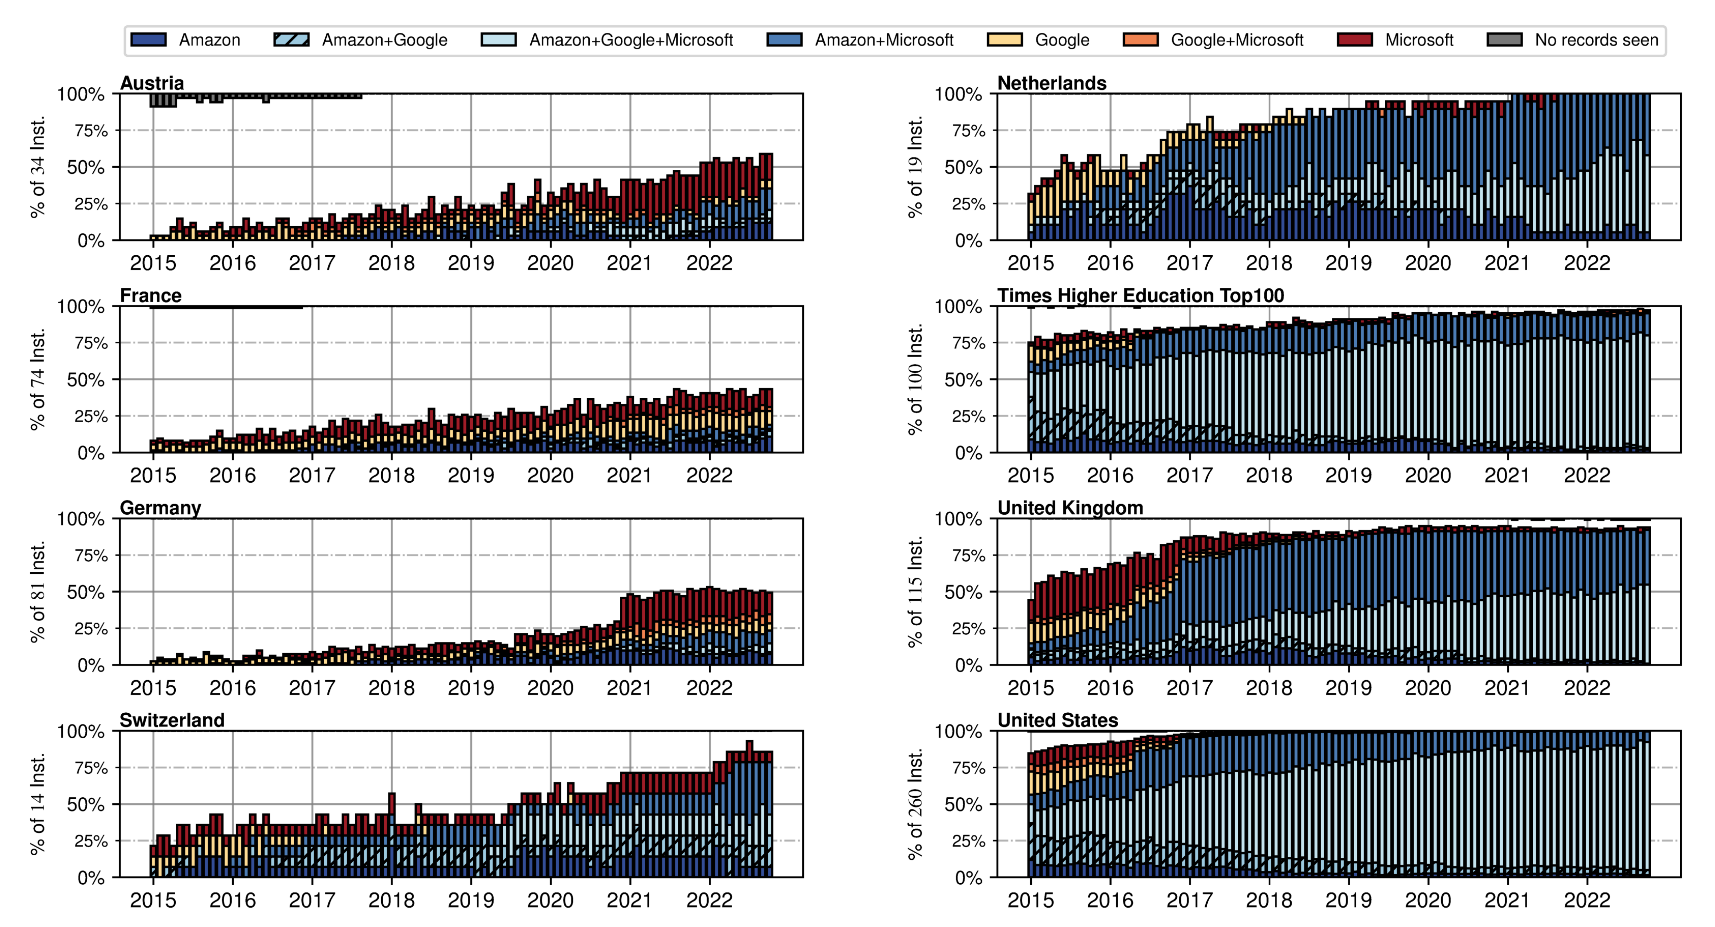
\includegraphics[width=0.9\textwidth]{img/digitalization_erupean_hei_fiebig.png}
  \caption{\centering{Increasing use of external cloud providers by European universities from January 2015 to October 2022 \cite{fiebig_heads_2023}.}}
  \label{fig:digitalization_european_universities}
\end{figure}

Some existing and ongoing studies agree on the potential risks and long-term implications that digitalization imposes on educational institutions. They suggest that self-hosting practices could be a viable solution for universities to regain control over their digital infrastructure. The use of Free/Libre Open Source Software (FLOSS), at least for critical digital services, can enhance transparency and provide guarantees regarding the proper use of data. FLOSS adoption and self-hosting represent an opportunity for universities to play an active role in developing and maintaining solutions that align with their institutional needs. Moreover, contributing to and adopting FLOSS solutions can help build strong internal capacity and foster greater technological independence and autonomy. Clearly, self-hosting requires significant long-term investments, and the optimized cost-efficiency implied by cloud resource dynamic allocation and the pay-as-you-go model is not comparable in the short term. However, as internal personnel expertise grows, the outcome may prove a more sustainable option, potentially reducing costs over time \cite{fiebig_heads_2023}. Additionally, research encourages universities to prioritize solutions that promote pedagogical values and view open-source solutions and self-provision as an ethical alternative to the current trend.

In support of the research, Huang M., in his extensive study involved some northwestern European universities, confirmed that economic considerations still represent a major factor in DETs procurement, often justified by limited financial resources and a lack of human resources. Although environmental sustainability is considered an important requirement, the lack of environmental impact metrics and the challenges in obtaining data tend to overshadow it, leading institutions to prioritize other sustainability aspects \cite{huang_building_2023-1}.

It is evident that there is a need for a critical shift in edtech procurement. Further research could make a major contribution to addressing and analyzing the new challenges and the ethical concerns created by digital education technologies \cite{teras_post-covid-19_2020}. 

\section{Sustainability dimensions for DETs}
\label{sec:2.3_sustainability_dimensions_DETs}
Among the hundreds of definitions associated with sustainability, the concept of sustainable development, introduced by the Brundtland Report \cite{are_1987_nodate}, remains the most widely recognized and accepted. It is defined as "meeting the needs of the present without compromising the ability of future generations to meet their own needs". However, its context-specific nature prevents it from being reduced to a single, universal definition. Sustainability is often depicted as an interdependent relationship between three distinct dimensions: economic, social, and environmental \cite{purvis_three_2019}. The foundational concept underlying the three-pillar model is the necessity of balancing the three aforementioned dimensions, in contrast to the assumption that economic growth alone can ensure sustainability and long-term prosperity. Treating these dimensions as isolated concerns can have detrimental effects. Disregarding the environmental dimension can result in increased pollution, excessive resource consumption, and climate change while exacerbating social inequalities. On the other hand, ignoring the social dimension may affect social well-being, contributing to weakened economic productivity and subsequent environmental degradation due to unsustainable practices.

A closely related popular framework that applies sustainability principles in a business-oriented context is Elkington's Triple Bottom Line (TBL), which extends the traditional bottom line of financial performance by incorporating social and environmental factors (People, Planet, Profit - 3P) \cite{correia_sustainability_2019}. The model encourages organizations to integrate corporate social responsibility initiatives into their decision-making processes, such as ensuring people's welfare as well as their contribution to the community. The model also incentivizes minimizing the environmental footprint, addressing the problems of energy consumption, waste production, and the use of natural resources. However, the framework is primarily designed to evaluate business performance in terms of measurable output and has been criticized for favoring the economic dimension over the social and environmental ones. This often leads companies to superficially address sustainability while maintaining a primary focus on profit.

\begin{figure}[ht!]
  \centering
  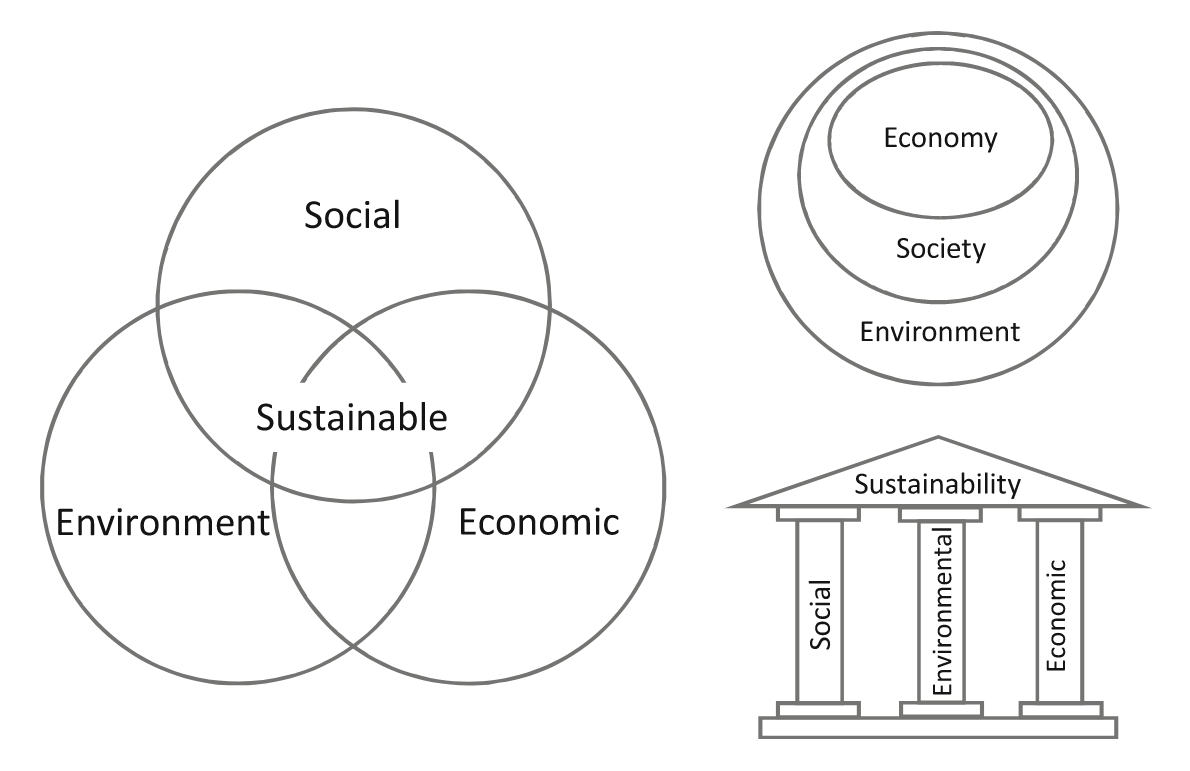
\includegraphics[width=0.6\textwidth]{img/three_pillars_model.png}
  \caption{\centering{Common representations of sustainability: (from left) overlapping circles, structural pillars, and a hierarchical model \cite{purvis_three_2019}.}}
  \label{fig:three_pillars_model}
\end{figure}

It is evident that the TBL model is not well suited for assessing the sustainability of digital education technologies. The selection process for education technologies requires a broader evaluation of social and ethical aspects that go beyond the business-oriented focus of this framework. Moreover, key factors such as pedagogical effectiveness and accessibility do not align with the dimensions proposed by the triple bottom line. Additionally, its emphasis on profitability contrasts with the financial dynamics of universities, which are geared toward economic feasibility and resource management.

The holistic approach suggested by the three-pillar concept represents a more appropriate solution for the selection process of digital education technologies. By extending the traditional framework to include pedagogical and technical dimensions, it provides a more comprehensive evaluation method that aligns with the specific needs of higher education institutions. This expanded model will serve as the foundation for the framework developed in this thesis, ensuring a sustainability-driven approach that aims to balance all the dimensions at stake.
      \newpage
      \ % The empty page
      \newpage
      
      \chapter{DETs Selection Framework}
\label{cha:3_framework}
This chapter describes the structure of the framework, identifies the stakeholders involved and their roles, and defines the assessment methodology and sustainability dimensions along with their respective indicators. A summary table is provided for each dimension, while the complete table can be found in Appendix \ref{cha:attachment_overleaf_comparison}.

Section \ref{sec:3.1_framework_structure} introduces the framework describing its structure. Section \ref{sec:3.2_stakeholders} describes the stakeholders involved and provides a high-level schema, while Section \ref{sec:3.3_assessment} defines the assessment methodology. Finally, Section \ref{sec:3.4_sustainability_dimensions} defines the sustainability dimensions and their indicators.

\section{Introduction to the framework}
\label{sec:3.1_framework_structure}
In recent years, the continuous integration of software and hardware solutions into learning, teaching, and administrative activities has led to the problem of selecting digital education technologies. As discussed in the previous chapters, this process seems to take place with little to no consideration of sustainability, while economic factors remain the dominant driving force. Recent studies have highlighted that the absence of evaluation criteria, along with common challenges such as limited financial resources, significantly impacts the procurement of sustainable digital education technologies \cite{huang_building_2023-1}. In addition, research literature concurs on the multi-dimensional nature of sustainability and its impact on the long-term viability and effectiveness. The purpose of the framework is to address this gap by providing a structured approach to evaluating whether DETs meet the sustainability requirements of higher education settings. The model is designed to assist decision makers in making informed choices that balance trade-offs across all the involved dimensions. \\
%As shown in the figure (insert figure), the framework consists of:
The framework consists of:
\begin{itemize}[noitemsep, topsep=4pt, parsep=0pt, partopsep=0pt]
    \item A set of stakeholders with distinct roles
    \item A set of interrelated dimensions, each assessed through a set of indicators
    \item Distinct sets of indicators (one per dimension), each associated with specific metrics and assessment methods
\end{itemize}
%Due to the wide range of digital technologies - both hardware and software - that could be assessed by this framework, it allows a versatile approach where some indicators could be re-assessed in a different dimension than the starting one, at the discretion of who is in charge of the selection process. Furthermore, some indicators may fit better to certain circumstances and the freedom to exclude some indicators is granted if the application is particularly complex or not possible at all.
Given the wide range of digital technologies, both hardware and software, that this framework can assess, it offers a versatile approach. Certain indicators may be reassessed under a different dimension instead of their initial one, at the discretion of those responsible for the selection process. Furthermore, some indicators may be more suitable for specific circumstances, and the flexibility to exclude certain indicators is granted when their application is particularly complex, counterproductive, or not possible at all. Examples of digital education technologies are listed in Table \ref{tab:examples_DETs}, grouped by category.

Each component of the framework will be further discussed in its respective section.

\begin{table}[ht!]
    \centering
    % \small
    \scriptsize
    % \tiny
    % \footnotesize
    \renewcommand{\arraystretch}{1.5} % Adjust row height
    \begin{tabular}{|>{\centering\arraybackslash}m{6.5cm}|>{\centering\arraybackslash}m{5.5cm}|}
        \hline
        \textbf{Category} & \textbf{Education technology} \\
        \hline
        \multirow{3}{*}{Cloud computing and virtual machines} & Amazon AWS  \\
        \cline{2-2}
        & Azure \\
        \cline{2-2}
        & Heroku \\
        \hline
        \multirow{3}{*}{Communication} & Discord  \\
        \cline{2-2}
        & Slack \\
        \cline{2-2}
        & Skype \\
        \hline
        \multirow{3}{*}{Gamification and Quiz} & Kahoot! \\
        \cline{2-2}
        & Mentimeter \\
        \cline{2-2}
        & Socrative \\
        \hline
        \multirow{3}{*}{Generative AI} & ChatGPT  \\
        \cline{2-2}
        & PaperPal \\
        \cline{2-2}
        & Writefull \\
        \hline
        \multirow{4}{*}{Learning management systems} & Blackboard \\
        \cline{2-2}
        & Canvas \\
        \cline{2-2}
        & Google Classroom \\
        \cline{2-2}
        & Moodle \\
        \hline
        \multirow{2}{*}{Massive Open Online Courses (MOOCs)} & Learnn \\
        \cline{2-2}
        & Udemy \\
        \hline
        \multirow{2}{*}{Video streaming} & Kaltura \\
        \cline{2-2}
        & Youtube \\
        \hline
        \multirow{5}{*}{Video conferencing} & Big Blue Button (BBB) \\
        \cline{2-2}
        & Google Meet \\
        \cline{2-2}
        & Microsoft Teams \\
        \cline{2-2}
        & Webex \\
        \cline{2-2}
        & Zoom \\
        \hline
        \multirow{3}{*}{Writing} & Google Documents \\
        \cline{2-2}
        & Microsoft Word \\
        \cline{2-2}
        & Overleaf \\
        \hline

    \end{tabular}
    \caption{Categories of DETs considered in framework development and examples}
    \label{tab:examples_DETs}
\end{table}

%Three of the five dimensions—Economic, Social, and Environmental—are derived from the widely recognized three Pillars of Sustainability concept, ensuring alignment with fundamental sustainability principles. These dimensions capture the financial feasibility, societal impact, and ecological footprint of DETs, respectively. The Pedagogical dimension is adapted from previous research in educational technology sustainability, recognizing the critical role of digital tools in supporting learning effectiveness and teaching methodologies.  Each dimension is assessed through a set of carefully selected indicators, which provide measurable criteria for evaluation. These indicators, in turn, are associated with specific metrics and assessment methods to ensure a structured and objective evaluation process. 

\section{Stakeholders}
\label{sec:3.2_stakeholders}
The stakeholders taking part in the dynamics of the framework are the following:
\begin{itemize}[noitemsep, topsep=4pt, parsep=0pt, partopsep=0pt]
    \item \textbf{Student and teachers} - Students and teachers, but also researchers, employees, and anyone who makes use of DETs and services offered by the university.
    \item \textbf{Provider} - The vendor or organization that offers its products to the university. It is expected to act as the service provider or as the cloud provider.
    \item \textbf{University} - IT specialists, IT heads, and all those who represent the institution and contribute to the DETs selection process.
\end{itemize}
\noindent

The high-level view of the framework illustrated in Figure \ref{fig:framework_stakeholders} describes how the stakeholders are involved in sustainability. The figure emphasizes how the university's control over many aspects of sustainability is reduced in the presence of an external provider. When dealing with FLOSS or self-hosting, higher education institutions assume the role of the provider, gaining stronger control over every dimension and limiting the impact of the provider.

% \begin{figure}[ht!]
%   \centering
%   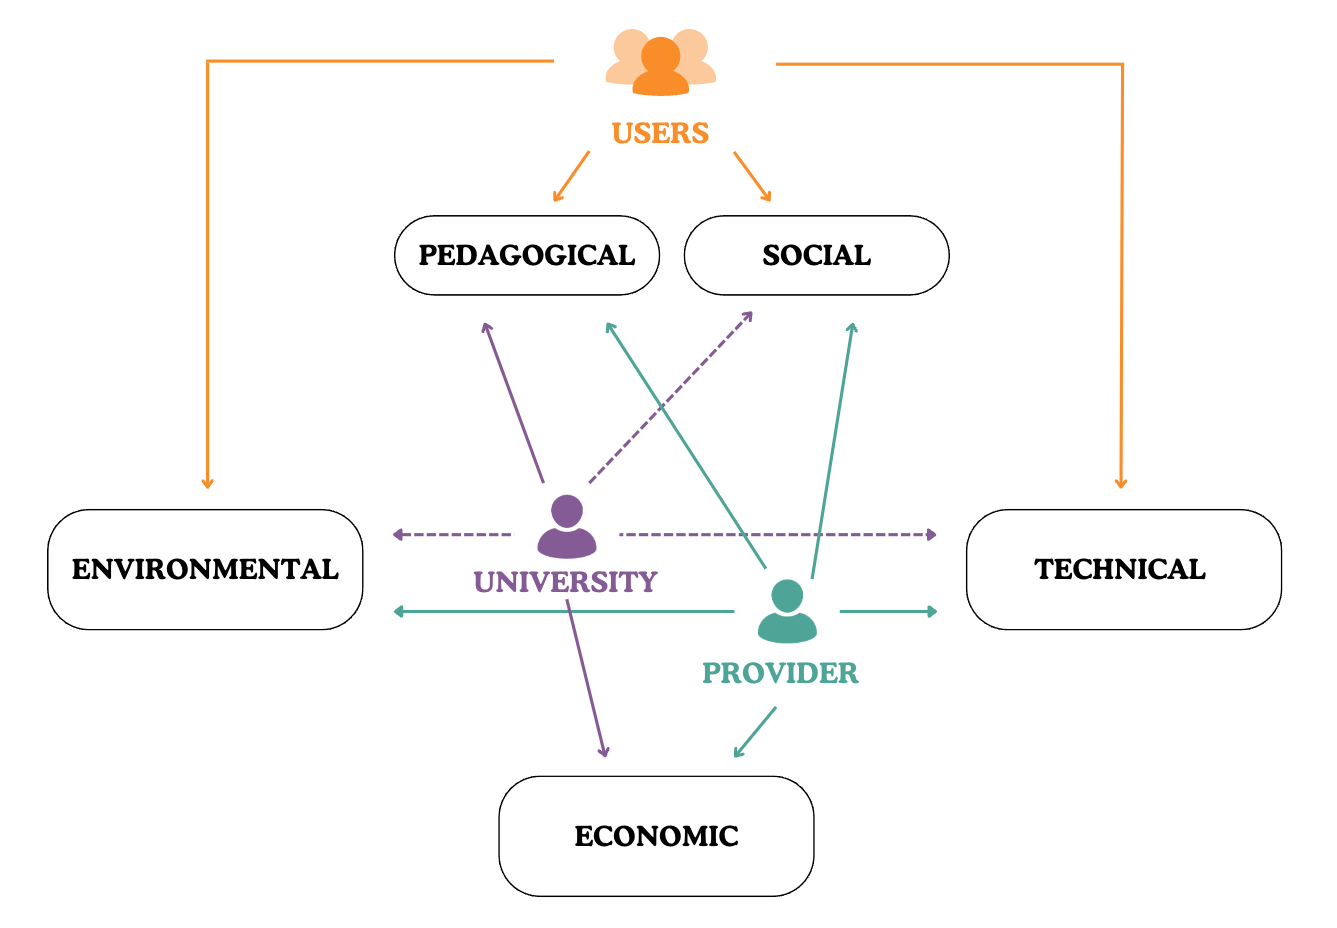
\includegraphics[width=0.85\textwidth]{img/framework_roles.png}
%   \caption{\centering{Actors and sustainability dimensions}}
%   \label{fig:framework_roles}
% \end{figure}

\begin{figure}[ht!]
  \centering
  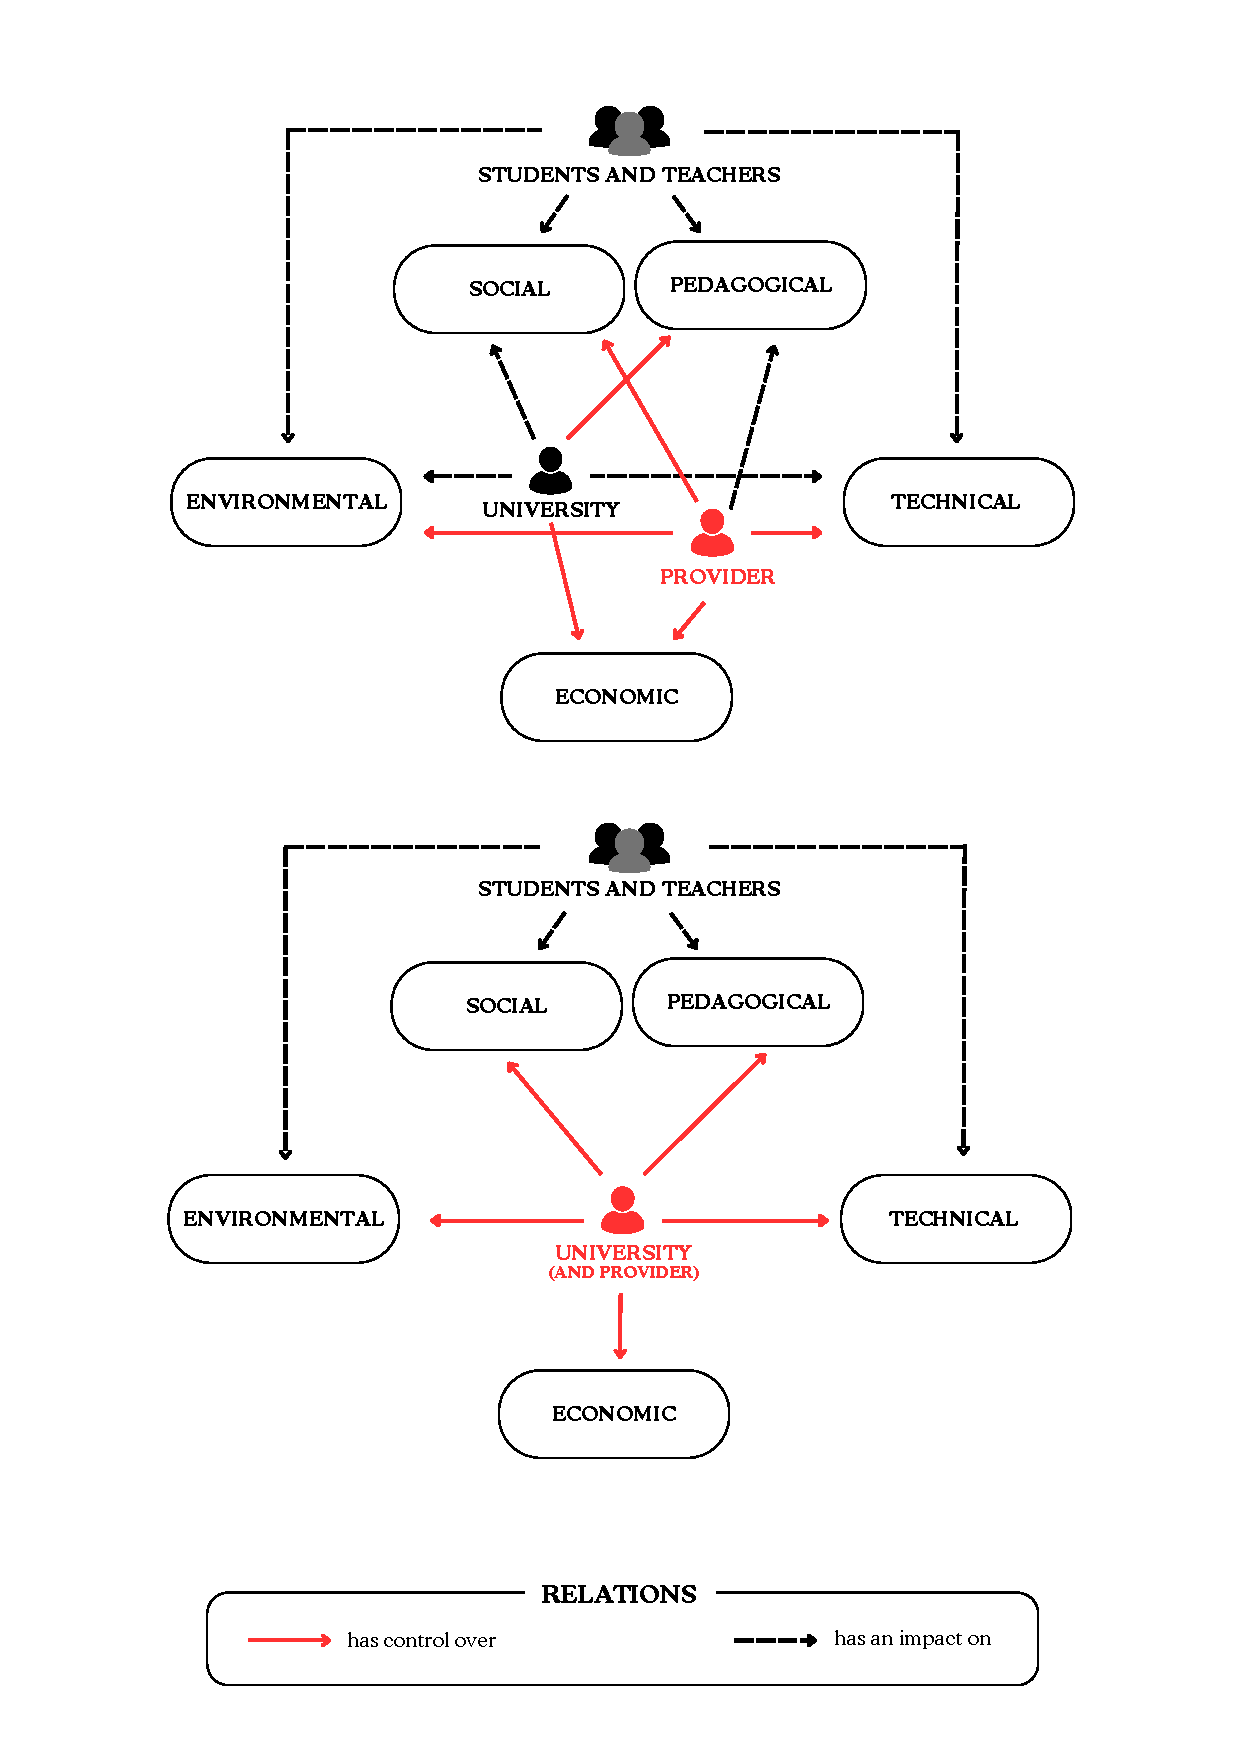
\includegraphics[width=0.95\textwidth]{attachments/framework_stakeholders.pdf}
  \caption{\centering{Relations between stakeholders and sustainability dimensions. The upper section illustrates these relations when the provider acts as the service provider, while the lower section shows them when the university assumes this role. }}
  \label{fig:framework_stakeholders}
\end{figure}
% Schema con controllo e impatti con due colori diversi
% Uno che mostra con provider e uno senza
% cambiare utenti con studenti e insegnanti

\section{Assessment methodology}
\label{sec:3.3_assessment}
To systematically assess the sustainability of digital education technologies, the framework employs a revised traffic-light rating system that categorizes each indicator into three levels: Red, Yellow, and Green. This choice is based on the idea that the traffic-light system provides an intuitive and immediate way to interpret the performance of each indicator. The meaning of the levels is defined as follows:
\begin{itemize}[noitemsep, topsep=4pt, parsep=0pt, partopsep=0pt]
    \item \textbf{Red light} - An indicator is classified as red when the technology under consideration does not meet the minimum requirement.
    \item \textbf{Yellow light} - A yellow light is assigned when the DET meets a minimum acceptable threshold for the indicator examined. This classification highlights the need for significant improvement, but it can also represent a situation of uncertainty in which further investigation is required.
    \item \textbf{Green light} - A green light confirms that the assessed DET is fully aligned with the indicator's requirement.
\end{itemize}

For comparative analysis between different DETs or multiple versions of the same DET, the results are numerically converted into a scoring system, where \textbf{red} equals -1, \textbf{yellow} equal 0, and \textbf{green} equals 1. The total score serves as a comparative metric, facilitating the ranking of different solutions based on their overall sustainability performance. However, when assessing an education technology without comparable alternatives or when evaluating the adoption of a new DET, the total score may lack contextual significance. In such cases, the overall distribution of traffic-light indicators provides a clearer qualitative evaluation, highlighting areas of strength and potential improvement without reducing the assessment to a single numerical value. Clearly, if a dimension lacks green lights or if the majority of the indicators turn red, the adoption of the technology is highly discouraged.


\section{Sustainability dimensions}
\label{sec:3.4_sustainability_dimensions}
The framework is built upon a multi-dimensional approach that integrates established sustainability principles with domain-specific considerations, i.e., pedagogical in the context of education and technical in the context of digital technologies. The first set of dimensions - economic, social, and environmental - are derived from the widely recognized three pillars of sustainability model, ensuring alignment with fundamental sustainability principles. The pedagogical dimension is adapted from previous research in sustainable education and a critical analysis of digitalization. Finally, the technical dimension is derived from the software-specific sustainability frameworks developed by Lago et al. \cite{lago_framing_2015} and Andrikopoulos et al. \cite{andrikopoulos_software_2021}, with modifications to accommodate broader technological solutions such as those of edtech. 

The following sections detail each dimension, its relevance, and the indicators used for assessment.

\subsection{Economic dimension}
The economic dimension represents the economic feasibility of a technology used in the context of higher education throughout its entire lifecycle. Budgetary and financial constraints exert a strong influence over the selection process, determining cost efficiency as a central theme.
This perspective builds upon the sustainability-aware framework proposed by Andrikopoulos et al. \cite{andrikopoulos_software_2021}, which defines economic sustainability in Software as a Service (SaaS) by emphasizing the maximization of return of expenses. However, since this model was specifically designed for SaaS, it requires adaptation when applied to a wider range of digital education technologies.
From Andrikopoulos’ framework, we can derive return of expanses as a fundamental indicator, as well as the related indicators of provisioning and scaling policies. By enhancing this aspect, cost efficiency is not only confined to expenditures reduction but also encompasses the optimization of resource allocation to ensure sustainability.
Furthermore, following the insights of Fiebig et al. \cite{fiebig_heads_2023} and Angeli et al. \cite{angeli_conceptualising_2022}, it is crucial to account for the economic implications of discontinuing a technology or migrating to alternative ones, confirming the need for indicators that examine exit costs and the influence of vendor synergies (i.e. lock-in). These factors can significantly impact the institution's ability to transition between different solutions and must be considered in the selection process.
This set of indicators is designed to prioritize the long-term economic viability of a technology over its short-term cost benefits.

\subsubsection{Return of Expenses}
The concept of return of expenses (RoE) can be defined as the degree of efficiency in consuming resources, such as cloud, hardware, and monetary assets, with respect to the generated revenue \cite{andrikopoulos_software_2021}.
During the selection process, universities may encounter two different scenarios:
\begin{enumerate}[noitemsep, topsep=4pt, parsep=0pt, partopsep=0pt]
    \item The technology is already in use, served on-premise or through an external provider, and there is an intention to migrate towards an alternative.
    \item The technology has not yet been adopted.
\end{enumerate}
In the first case, RoE serves to estimate the degree of success and the economic benefits that would result from migrating the existing technology to an alternative solution.
In the second case, the institution must define what constitutes "generated revenue" within its domain and establish an acceptable threshold. For example, this indicator should help answer the following questions:
\begin{center}
    \textit{“How likely is the DET to be adopted by users?”} \\
    \textit{"How likely is the DET to remain in use over time?"}
\end{center}
When applied to software solutions, this indicator is particularly useful in cases such as comparing cloud-based tools with technologies available exclusively on-premises. Furthermore, if RoE is used to compare different deployment models of the same technology, the generated revenue may be similar across cases and can therefore be excluded from the evaluation process. However, RoE is inherently limited by the vast range of technologies it can assess, necessitating a more specific definition tailored to each case. Developing systematic evaluation methods to estimate return of expenses remains an open area for future research. The exclusion of this indicator from the study was not considered, as even a high-level analysis can provide valuable insights for its assessment.

\subsubsection{Provisioning}
The provisioning indicator aims to measure the resources allocated, either cloud-based or local, in relation to the expected resources required to ensure the proper operation of the service. Despite its technical nature, the provisioning indicator is placed within the economic dimension as it directly impacts cost-efficiency. In fact, resources represent a significant cost factor that cannot be ignored, and minimizing energy waste and underutilized resources is essential to reduce costs. Typically, an incorrect estimation of the required resources leads to two possible outcomes: over-provisioning and under-provision. Over-provisioning leads to unnecessary expenses due to unused resources, while under-provisioning leads to performance degradation and potential loss of generated value (i.e. university community cannot make use of the technology).
This indicator is evaluated through the Quality of Provisioning metric, defined as:
\[
\text{Quality of Provisioning (QoP)} = \frac{\text{Allocated Resources}}{\text{Used Resources}}
\]
The QoP indicator is designed to facilitate the comparison of different deployment models, generating measures for many provisioning cases that are later correlated with the cost of the allocated resources. The result is the expected cost per user. It is evident that when comparing local infrastructure with cloud-based solutions, the indicator tends to favor cloud resources. This is because cloud providers distribute costs across the user base, leading to optimized resource allocation that is hardly achievable in other contexts. Additionally, in the case of cloud-based solutions, detailed information about provisioning is often not disclosed, as resources are abstracted and offered at a fixed price rather than being transparently allocated based on actual usage.

This indicator can also be later reiterated in the context of technical sustainability.

\subsubsection{Scaling policies}
The scaling policies indicator integrates the provisioning indicator by examining how resources are managed once provisioned. While provisioning assesses the efficiency of resource allocation, scaling policies analyze how these resources are adjusted over time.
Except in special cases, the on-demand approach is preferred over the always-on model, which tends to generate more waste. Ideally, the system should always be able to compensate for the load. The effectiveness of the indicator is bound to the technical characteristics of the technology, as different architectures and infrastructures impose varying constraints and possibilities for resource scaling. This indicator is evaluated through the same metric as the previous one, which should be reiterated according to the scaling policy to reflect the related costs. Alternatively, the average percentage of wasted resources (\%) could provide valuable insights.

\subsubsection{Vendor synergies (lock-in)}
Vendor synergies refer to the advantages and operational efficiencies that emerge when universities integrate multiple digital services and infrastructures from a single vendor. Cloud providers often offer bundled services with advantageous pricing models, which are highly integrated into the vendor ecosystem. These practices often lead to reduced management complexity and potentially lower costs, but they may also enable lock-in mechanism and increased dependence on proprietary standards and services \cite{komljenovic_rise_2021}\cite{fiebig_heads_2023}. For example, Google Workspace and Microsoft 365 are highly integrated platforms that provide several solutions within the same ecosystem. Even if universities host services on their own digital infrastructure, they may still rely on proprietary standards and integrations, making it difficult to migrate to alternative solutions without significant costs and effort.
This indicator aims to identify and quantify vendor synergies that may impact the migration process away from the vendor’s ecosystem. To develop a metric, the institution should analyze the technology to identify evidence of lock-in and soft lock-in practices. An acceptable level is when the impact of synergies is manageable during the migration process, while soft lock-in can be neglected if its influence is minimal\footnote{In this study, soft lock-in refers to all the features and characteristics that enhance the technology without imposing legal or technical restrictions.}.

\subsubsection{Exit costs}
The purpose of the exit cost indicator is to quantify the effort, and thus the cost, of moving either toward an external provider or to the university's digital infrastructure. In the first case, the total cost of the migration consists of the expense of IT staffing and the price agreed with the new vendor. In the second case, other complexities come into play, such as the cost of upgrading the internal infrastructure (both hardware and software components) and the procurement of new technical staff.       

\bigskip

\begin{table}[ht!]
    \centering
    \small
    % \scriptsize
    % \tiny
    % \footnotesize
    \renewcommand{\arraystretch}{1.5} % Adjust row height
    \begin{tabular}{|>{\centering\arraybackslash}m{3cm}|>{\centering\arraybackslash}m{3.1cm}|>{\centering\arraybackslash}m{2.9cm}|>{\centering\arraybackslash}m{2.9cm}|>{\centering\arraybackslash}m{2.9cm}|}
        \hline
        \textbf{Indicator} & \textbf{Metric} & \textbf{Red light} & \textbf{Yellow light} & \textbf{Green light} \\
        \hline
        Return of Expenses & To be defined within the institution & Low or absent generated value & Acceptable generated value & Optimal generated value \\
        \hline
        Provisioning & Quality of Provisioning & High cost per user & Acceptable cost per user & Low cost per user \\
        \hline
        Scaling policies & Waste of resources & High waste & Acceptable waste & Low waste \\
        \hline
        Vendor synergies & Vendor make use of lock-in practices & Legal/technical restrictions, proprietary standards, etc. & Soft lock-in & Negligible or no soft lock \\
        \hline
        Exit costs & Total expenses of exit/migration & High costs & Acceptable costs & Very low costs \\
        \hline
    \end{tabular}
    \caption{Summary of the economic indicators}
    \label{tab:summary_economic_indicators}
\end{table}

\subsection{Technical dimension}
Technical sustainability is the dimension that requires software and hardware systems to remain operational, efficient, and adaptable over time. This dimension lays its foundations on key principles derived from distributed systems theory, such as dependability and maintainability \cite{tanenbaum_distributed_2006}. In this framework, the concept of dependability is not treated as a mere technical definition, but is integrated with the concept of Quality of Service (QoS) presented by Andrikopoulos et al. \cite{andrikopoulos_software_2021}. QoS relates to how users perceive the system and its ability to fulfill their expectations, while dependability refers to the system's ability to deliver its functionality in depth of time. QoS relies on dependability, incorporating its operational and architectural aspects, like availability, reliability, and scalability, which are reshaped according to users' need. Maintainability, on the other hand, remains faithful to its classical definition, requiring ease and efficiency in updating, upgrading, and repairing the system. These two principles intersect in the operational indicator of adaptability, which is essential for the long-term viability of the system. Typically, private companies withhold their system specifications from the public. Thus, when dealing with external providers who are not likely to share such information, the assessment of technical sustainability is limited to a high-level perspective.    

\subsubsection{Availability}
In the context of the tech business, availability is often defined as "the ability to be operational at all times, from anywhere, using any device"\footnote{Lucidchart - \href{https://www.lucidchart.com/blog/reliability-availability-in-cloud-computing}{https://www.lucidchart.com}}. Although this definition applies to web technologies, it suffers the influence of the cloud computing model. In the wider context of education technologies, a more appropriate definition is "the ability to be operational at a given time"\footnote{Atlassian - \href{https://www.atlassian.com/incident-management/kpis/reliability-vs-availability}{https://www.atlassian.com}}. This implies that, depending on the DET, it is not required to be always available, but rather to be available when needed. For example, a video conferencing tool used exclusively to host lectures has no reason to be available before and after the class schedule. Typically, high availability is required for critical services and systems, such as administrative tools and email services. This indicator is evaluated through the availability percentage metric (also known as uptime percentage), defined as:
\[
    \text{Availability percentage} = \frac{\text{Uptime}}{\text{Total time}} \times 100
\]
Clearly, this metric may be difficult to estimate during the selection process, but for DETs already provided as a service, availability measurements can be conducted based on historical performance data. An acceptable level of availability should be defined based on the specific DET under evaluation.

\subsubsection{Reliability}
Similarly to the previous indicator, reliability is defined as "the probability that a system or component will perform its intended function without failure under specified conditions for a given period". This implies that although a certain DET is available, it is not necessarily reliable. 

Different metrics have been developed to assess reliability. One of the most popular is the error rate metric, expressed as a percentage:
\[
    \text{Error rate} = \frac{\text{Number of failed operations}}{\text{Total number of operations}} \times 100
\]
Like availability, high reliability is required for critical services and systems, such as remote proctoring software or learning management systems with assessment features.

\subsubsection{Scalability}
As defined in distributed systems theory, the scalability of a system refers to its ability to increase or decrease its scale in terms of size, geographic distribution, and administrative span \cite{tanenbaum_distributed_2006}. In this framework, the focus is on size, since it determines how likely a technology is to accommodate new users, data, and resources. Among the dependability attributes, scalability represents the most difficult to examine, as cloud providers typically abstract the underlying system from users. To evaluate scalability, two cases can be distinguished:
\begin{itemize}[noitemsep, topsep=4pt, parsep=0pt, partopsep=0pt]
    \item DET is offered by a vendor - The indicator is generally not applicable, since the complexity is delegated to the external provider. However, for cloud-based solutions, monitoring metrics can offer useful insights, such as average response time.
    \item DET is deployed as self-hosted - The study of the technology should determine whether it sufficiently supports scalability techniques.
\end{itemize}
For example, if a DET does not support either horizontal or vertical scaling, the indicator will result in a red light. Conversely, if a DET supports load balancing, as well as both vertical and horizontal scaling, the indicator will result in a green light.

\subsubsection{Maintainability}
Maintainability is a key principle in the context of systems and software architectures. It can be seen as a set of fundamental properties, such as availability, upgradability, and repairability\footnote{Microsoft page on GitHub - \href{https://microsoft.github.io/code-with-engineering-playbook/non-functional-requirements/maintainability/}{https://microsoft.github.io/code-with-engineering-playbook/}}. Given their significance, each of these properties give rise to an indicator. In this framework, maintainability is confined to the ability of a software or a system to be easily configured, updated, and upgraded. In addition to the installation and distribution methods, the quality of the documentation and support plays a crucial role in achieving a satisfactory level of maintainability. To obtain a good score, ease and efficiency in installing and updating the software are required.

\subsubsection{Adaptability}
The concept of adaptability varies depending on the subject: software architectures and system architecture. The former is built upon extensibility, flexibility, tunability, and fixability \cite{fayad_aspects_1996} and refers to the willingness of software architectures to accept changes without significant code rewrites or architecture redesign. Adaptable software is likely to support new features and changes without extensive rework, allow integration of new and external components, and facilitate migration to other systems. The latter refers to the capability of a system to manage changes in hardware and software components while continuing to fulfill its requirements \cite{tanenbaum_distributed_2006}. Adaptable systems promote modularity and support the integration of new hardware and software technologies.

Research literature suggests some metrics for this indicator, such as those proposed by Subramanian et al. at the University of Texas at Dallas \cite{subramanian_metrics_2001}. However, the assessment requires in-depth knowledge of the software architecture or system architecture and inevitably becomes more complicated when external solutions are adopted. In this study, the adaptability indicator is limited to verifying how a given solution integrates within the institution's infrastructure (e.g., Single Sign-On) and how it interacts with third-party services. To obtain a green light, integration with both is mandatory.  

\subsubsection{Repairability}
Software repairability (or fixability) is a multifaceted attribute, generally considered a subset of maintainability. It is defined as the ability to resolve defects without introducing unintended issues elsewhere. From a broader perspective, software repairability is not limited to fixing bugs and inaccuracies in the code, but also includes addressing errors and malfunctions that affect functionality. The disruption of a cloud service is not necessarily related to a software issue. Factors such as connectivity problems or underlying infrastructure failures can also be responsible. Therefore, software repairability refers to interventions within the software itself, either through code modifications or control tools, and to related components that may contribute to malfunctions, ensuring the recovery of availability and reliability when they are compromised.

The repairability indicator, when applied to software, results in a green light when both code changes (i.e., open-source) and direct intervention on operational factors are permitted. It results in a yellow light when code modifications are not allowed, but it is still possible to take actions on related factors. Finally, it results in a red light when no repair interventions are possible.

The definition of hardware repairability, instead, is inspired by the French Repairability Index, which aims to assign a score that quantifies the ease of repair for electrical and electronic devices\footnote{French Repairability Index - \href{https://repair.eu/it/news/the-french-repair-index-challenges-and-opportunities/}{https://repair.eu/}}. To be classified as repairable, hardware should be accompanied by repair manuals and guidelines and should be designed for simple assembly and disassembly. Additionally, spare parts should be available, easy to find, and reasonably priced. Finally, another factor that ensures better repairability is the absence of artificial barriers, such as soldered components.

The repairability indicator, when applied to hardware components, provides a score that ranges from 1 to 5, where 1 indicates poor repairability and 5 indicates high repairability.

\bigskip

\begin{table}[ht!]
    \centering
    \small
    % \scriptsize
    % \tiny
    % \footnotesize
    \renewcommand{\arraystretch}{1.5} % Adjust row height
    \begin{tabular}{|>{\centering\arraybackslash}m{3cm}|>{\centering\arraybackslash}m{3.1cm}|>{\centering\arraybackslash}m{2.9cm}|>{\centering\arraybackslash}m{2.9cm}|>{\centering\arraybackslash}m{2.9cm}|}
        \hline
        \textbf{Indicator} & \textbf{Metric} & \textbf{Red light} & \textbf{Yellow light} & \textbf{Green light} \\
        \hline
        Availability & Uptime (\%) & \multicolumn{3}{c|}{To be defined based on the DET} \\ 
        \hline
        Reliability & Error rate (\%) & \multicolumn{3}{c|}{To be defined based on the DET}  \\
        \hline
        Scalability & Scalability support & Little to no support for scalability techniques & Partial support for scalability techniques, with limitations in the long-term & Support scalability techniques \\
        \hline
        Adaptability & Degree of integration within university infrastructure and third-party components & No integration & Partial integration (e.g., only SSO) & Full integration (university infrastructure and multiple third-party components) \\
        \hline
        Maintainability & Ease of configuration, updates, and upgrades & Difficult to configure/update; poor documentation and support & Moderate ease of installation and updates; limited documentation and support & Easy and efficient installation, configuration, and updates; comprehensive documentation and support \\
        \hline
        \multirow{2}{*}{Repairability} & Interventions allowed & No interventions allowed & Limited interventions allowed (e.g., only infrastructure)  & Full interventions allowed (code and infrastructure) \\
        \cline{2-5}
         & Ease of hardware repair (availability of manuals, ease of disassemble, availability of spare parts, price of spare parts, and artificial barriers) & Score: 1–2 (poor repairability) & Score: 3 (moderate repairability) & Score: 4–5 (high repairability) \\
        \hline
    \end{tabular}
    \caption{Overview of technical indicators}
    \label{tab:overview_technical_indicators}
\end{table}

\newpage % ATTENTION

\subsection{Social dimension}
Social sustainability is the dimension that fosters accessibility, inclusion, equity, and social interaction. Education technologies have the potential to achieve equal access to education for all, as well as to promote social well-being and reduce costs \cite{haleem_understanding_2022}. During the pandemic, the hasty introduction of digital tools without considering learners' nneds led to the marginalization of certain students due to unstable internet connections and a lack of access to digital devices \cite{haleem_understanding_2022}. Through social sustainability, institutions must ensure greater access to education, mitigating inequalities due to disabilities, low-income backgrounds, and geographical barriers. Additionally, as digital competencies become increasingly essential, institutions should also promote digital citizenship and the development of digital skills \cite{crick_covid-19_2021}.

The engagement of private companies in educational dynamics requires more effort to achieve social sustainability. A key aspect is the privacy risk related to the unchecked collection and use of sensitive data and learning analytics\cite{komljenovic_rise_2021}. Universities should safeguard the privacy of users, preventing the exploitation of student and faculty data for commercial purposes. From a more technical perspective, Andrikopoulos et al. suggest that the level of awareness also plays an important role in this dimension\cite{andrikopoulos_software_2021}. Vendors and universities are required to actively participate in sustainability efforts and to keep their community (i.e., university members) aware of the changes and decisions that affect it.

Finally, institutions should favor solutions that positively impact their personnel and students. The outsourcing trend is leading to a reduction of internal knowledge and capability, while universities should promote innovation and collaboration and achieve greater autonomy.

\subsubsection{Community awareness}
Awareness of the community is a concept adapted from the framework proposed by Andrikopoulos et al.\cite{andrikopoulos_software_2021}. Their intuition is to keep the community in the loop about changes and decisions affecting the system. By increasing the rate of awareness about the system, particularly regarding sustainability-related decisions, the community can be actively engaged in the efforts to increase the system's sustainability. This indicator assesses whether the university or the external provider keeps the university members informed about changes and their subsequent sustainability implications. This practice has the potential to improve transparency and should not be reduced to a mere change-log, which would inevitably result in a red light. To obtain a green light, awareness efforts must be driven by sustainability objectives.

\subsubsection{Involvement in sustainability}
Involvement in sustainability, rather than technology, is related to its owner. This indicator quantifies the distance between the provider (i.e., the university or the vendor) and a sustainability claim or study. The underlying idea is that if a sustainability study is directly attributable to the provider, then it can be considered actively engaged in sustainability efforts. Conversely, if finding a sustainability claim requires tracing multiple relationships through a network, the provider’s involvement is indirect and potentially superficial. For example, if the provider has no sustainability claims, it is not actively engaged. If the provider is associated with at least one organization that is involved in sustainability, then its distance is one "hop". Otherwise, at least one more hop is required, and becomes too distant to be considered involved in sustainability.

\subsubsection{Inclusion}
Digital education technologies should guarantee equal access for all learners regardless of disabilities, socioeconomic status, and geographical constraints \cite{haleem_understanding_2022}. To assess the inclusiveness of education technologies, two key aspects of accessibility should be considered:
\begin{itemize}[noitemsep, topsep=4pt, parsep=0pt, partopsep=0pt]
    \item Technological accessibility - Focuses on hardware and software requirements necessary for effective use.
    \item Inclusive usability – Focuses on how the technology accommodates individuals with disabilities and diverse learning needs.
\end{itemize}

DETs are required to achieve technological accessibility by limiting technological barriers, particularly in terms of hardware and software requirements, that may preclude some individuals from using them. In the case of remote learning, required bandwidth and processing power should be minimized, while device compatibility should be guaranteed as much as possible. For example, Zoom typically regulates video quality based on the available bandwidth. However, this could lead to inefficiency and a degraded user experience for those with low bandwidth or outdated devices.

Technological accessibility is addressed within the environmental dimension, since many of its aspects, such as performance optimization, technical requirements, and bandwidth usage, are closely connected to environmental concerns. Optimization has the potential to reduce energy consumption, while lower technical requirements can ensure wider compatibility with older devices, thus contributing to the reduction of electronic waste. In addition, efficient bandwidth usage can mitigate the impact of data transmission, which is particularly relevant given the increasing energy demands of cloud computing \cite{angeli_conceptualising_2022}.
As a result, technological accessibility is excluded from this indicator.

Inclusive usability, instead, encompasses compliance with accessibility standards and assistive features. In recent years there has been a strong focus on content accessibility, which has resulted in governments increasingly developing guidelines, such as the European Accessibility Act\footnote{European Commission - \href{https://commission.europa.eu/strategy-and-policy/policies/justice-and-fundamental-rights/disability/union-equality-strategy-rights-persons-disabilities-2021-2030/european-accessibility-act_en}{https://commission.europa.eu}} and the Americans with Disabilities Act (ADA)\footnote{ADA - \href{https://www.ada.gov/}{https://www.ada.gov}}, and enacting legislation to ensure compliance. Meanwhile, the World Wide Web Consortium (W3C) has developed the Web Content Accessibility Guidelines (WCAG), which is now the globally recognized standard for Web accessibility.

In this study, the European Accessibility Act is adopted as the minimum requirement, and thus WCAG 2.1 AA, since it is the referenced standard to ensure content accessibility. These guidelines are structured around four principles, requiring content to be perceivable (e.g., text alternatives, adequate contrast ratio), operable (e.g., keyboard accessibility, absence of timing restrictions), understandable (e.g., input assistance, readability of text), and robust (e.g., compatible with assistive technologies) \cite{acosta-vargas_challenges_2018}. Compliance with stricter guidelines such as WCAG 2.1 AAA or WCAG 2.2 is sufficient to get the green light.

Several methods could be adopted to assess this indicator:
\begin{itemize}[noitemsep, topsep=4pt, parsep=0pt, partopsep=0pt]
    \item Use of specific tools and browser extensions that produce availability reports, such as WAVE\footnote{WAVE - \href{https://wave.webaim.org/}{https://wave.webaim.org}} or ANDI\footnote{ANDI - \href{https://www.ssa.gov/accessibility/andi/help/install.html}{https://www.ssa.gov/accessibility/andi}}.
    \item Use of checklists for developers and manual testing.
    \item Review of accessibility reports published by the provider, if available.
\end{itemize}

\subsubsection{Privacy policy}
The privacy policy indicator states whether the collection and use of users' data is appropriate, legal and transparent. Typically, the greater the presence of data sub-processors, the less user have over their data.
To determine whether users' data is being processed appropriately, many aspects should be considered such as:
\begin{itemize}[noitemsep, topsep=4pt, parsep=0pt, partopsep=0pt]
    \item The content of privacy policies and terms of service.
    \item Clarity and readability of such policies.
    \item The amount of sub-processors involved in data processing.
    \item Security measures implemented to ensure data protection.
\end{itemize}
To score a yellow light, the minimum condition is compliance with the General Data Protection Regulation (GDPR)\footnote{General Data Protection Regulation - \href{https://gdpr-info.eu/}{https://gdpr-info.eu}}. To improve the score, data collectors and processors must limit data collection to only the necessary information, ensure that it is not exploited for commercial use, and provide clear and readable documentation. The assessment method primarily involves the study of the privacy policies, followed by the evaluation of readability using well-known readability indices, such as Flesch Reading Ease, Flesch-Kincaid, or Gunning Fog.     

\subsubsection{Capacity}
As mentioned in the previous sections, the outsourcing of digital infrastructure leads to the outsourcing of knowledge and a reduction in internal capabilities \cite{angeli_conceptualising_2022}. This indicator evaluates whether a technology is likely to generate internal capacity. Those responsible for the selection process should answer the following question:

\begin{center}
    \textit{"Does deploying or making this technology available require internal effort and knowledge?"}
\end{center}

\noindent
If the answer is "no", there is no need for internal knowledge about this technology, as management and operational activities are delegated to external entities. However, to achieve a good score, at least partial effort is required, ensuring that some level of internal knowledge about the technology is retained, such as in cases where an external service is integrated with the university's digital infrastructure. This guarantees a degree of transparency in its management and use.

\bigskip

\begin{table}[ht!]
    \centering
    \small
    % \scriptsize
    % \tiny
    % \footnotesize
    \renewcommand{\arraystretch}{1.5} % Adjust row height
    \begin{tabular}{|>{\centering\arraybackslash}m{3cm}|>{\centering\arraybackslash}m{3.1cm}|>{\centering\arraybackslash}m{2.9cm}|>{\centering\arraybackslash}m{2.9cm}|>{\centering\arraybackslash}m{2.9cm}|}
        \hline
        \textbf{Indicator} & \textbf{Metric} & \textbf{Red light} & \textbf{Yellow light} & \textbf{Green light} \\
        \hline
        Community awareness & Awareness of the community about the DET & No structured communication & Changes are communicated, but not for sustainability purposes & Users are proactively informed about changes, with a clear focus on sustainability \\
        \hline
        Involvement in sustainability & Distance to sustainability claim & Sustainability claims are absent or found through distant relations (more than 1 hop) & Sustainability claims are found through direct relations (1 hop) & Sustainability claims are directly attributable (0 hops) \\
        \hline
        Inclusion & Compliance with accessibility guidelines & No compliance & Compliance with EAA or WCAG 2.1 AA & Compliance with stricter guidelines (e.g., WCAG 2.1 AAA and 2.2) \\
        \hline
        Privacy policy & Protection and ethical use of user data; transparency on data collection and process & Not GDPR compliant; Insufficient readability & GDPR compliant; Readability may be improved & Ethical approach on users' data; Good readability \\
        \hline
        Capacity & Requires internal capacity and knowledge & Not required & Partially required & Required \\
        \hline
    \end{tabular}
    \caption{Summary of the social indicators}
    \label{tab:summary_social_indicators}
\end{table}

\newpage % ATTENTIION

\subsection{Pedagogical dimension}
The pedagogical dimension examines how digital education technologies support teaching and learning within higher education institutions. The introduction and ongoing expansion of education technologies have led to a continuous evolution in pedagogical practices, which have adapted with the aim of improving the learning experience and outcomes. Their rapid diffusion has also raised concerns about the preparation of students and teachers, as the lack of prior training negatively impacts the engagement with digital technologies \cite{schuetze_digitalization_2024}\cite{sokhulu_students_2021}. Universities should promote a proactive approach to education technologies and guarantee their usability.

As discussed in the previous chapter, DETs should support effective and accessible learning and should not be reduced to a basic integration of technologies into educational dynamics \cite{schuetze_digitalization_2024}\cite{teras_post-covid-19_2020}. Thus, this dimension ensures that DETs align with pedagogical best practices, such as the evidence-based instructional practices (EBIPs) \cite{lane_innovative_2020}. However, since pedagogical performance typically becomes evident only after the adoption of a DET, this dimension requires an assessment of the purpose and expected impact on teaching and learning before its implementation.
The indicators that shape this dimension are derived and adapted from both research literature and internal discussions with the supervisor. Since many aspects of pedagogical sustainability are the subject of ongoing research, this study proposes a set of indicators to conduct a high-level assessment. 

\subsubsection{Engaged with instructional practices}
Evidence-based instructional practices refer to those teaching strategies that are supported by hard research and proven to have a greater impact on learning outcomes compared to others. Universities should encourage the adoption of innovative and effective teaching strategies while also promoting research in this field. However, digital education technologies are often proposed as educational tools even when they are not grounded in solid pedagogical principles \cite{teras_post-covid-19_2020}. This indicator states whether a DET, or its owner, is actively involved in pedagogical research and contributes to the study of evidence-based teaching practices. A high score in this area would reflect the pedagogical principles underlying the technology. Conversely, a lower score indicates that the technology is simply adapted to the educational context.

\subsubsection{Usability}
Usability is a crucial factor in determining whether a digital education technology is accessible, efficient, and user-friendly. Unlike the inclusion indicator, which focuses on compliance with accessibility standards, usability evaluates the experience of users interacting with the technology. The usability of DETs affects learning effectiveness and the adoption rate within the institution. 
Poor usability may discourage its use since it could undermine academic productivity and lead to unnecessary cognitive load. 

To evaluate user interfaces and user experience, this study proposes an approach based on the widely recognized Nielsen's usability heuristics \cite{nielsen_enhancing_1994}, but usability assessments can be conducted using several frameworks. Those responsible for the selection process can adopt their preferred method. 

As an example, the usability indicator could be assessed using the following criteria:
\begin{itemize}[noitemsep, topsep=4pt, parsep=0pt, partopsep=0pt]
    \item Learnability - Basic tasks can be completed without external help, and tutorials and guidelines are available to users.
    \item Efficiency of use - Frequent actions should be completed without excessive time and effort.
    \item Error prevention and user control- The interface is designed to prevent users from making errors and, if necessary, provides hints and support for recovery. 
    \item Feedback and transparency of system status - The interface provides feedback on user actions, ensuring they are aware of the system's state at all times.
    \item Integrations and customization - Users are allowed to personalize their experience, integrating external tools or modifying the way the interface appears.
\end{itemize}

\noindent
Clearly this example cannot perform as effectively as popular frameworks, but it is sufficient to understand how usability was taken into account in the design and development of DETs. However, it is highly recommended to adopt a more structured and recognized framework.  
If preferred, the assessment can be done through alternative methods such as in-person usability tests, surveys, or automated tools, and can be iterated from a technical perspective.
The outcome must then be represented following the traffic-light model.

\subsubsection{Impact on education}
Impact on education is an indicator that estimates how the introduction of a digital education technology affects the learning process and the academic environment. This indicator considers several factors, such as the learning curve, compatibility with existing workflows, collaboration, improvement of output quality, and adaptability to the academic context. This indicator is developed by combining the outcomes of internal discussions and insights from research literature.

One of the most important aspects to consider when introducing a new DET is how easily students and teachers can familiarize themselves with it. A steep learning curve represents a significant barrier to adoption, since users will require training and effort to become productive. Intuitive DETs that can be effectively used with minimal training should be preferred, facilitating their adoption in the academic environment. Another important factor is the impact that the DET has on the existing workflow. Particularly when the introduction is driven by the willingness to replace an existing DET, institutions must be sure that the new technology brings improvements and increases efficiency instead of having a disruptive effect on the workflow. However, not all DETs are designed for educational purposes (e.g., Zoom) and may require adaptation to fit into learning dynamics. Universities need to carefully evaluate whether the DET is aligned with their needs. All these factors contribute to the effectiveness of a DET, which is reflected in the quality of academic output. The introduction of a new DET has to lead to improved learning outcomes, student engagement and knowledge retention, and not add complexity.

Since digital education technologies enable collaboration among students and instructors \cite{sokhulu_students_2021}, this indicator should account for whether the DET promotes collaboration by design, providing features that facilitate group work and student-teacher interactions, such as shared workspaces and real-time editing.  

If the DET aligns with all the aforementioned factors, then it will receive a green light. Otherwise, the institution should assess whether its impact is acceptable.

\subsubsection{Purpose}
The purpose is one of the most important indicators to consider in the selection process. Before adopting a technology, the institution must answer the following questions:
\begin{center}
    \textit{What is the problem we need to solve?} \\
    \textit{Could DETs solve the problem?} 
\end{center}
The outsourcing trend and the tendency of vendors to offer affordable bundled solutions lead to the introduction of unnecessary tools \cite{komljenovic_rise_2021}. This indicator can be seen as a kind of collective reflection, where those in charge of selecting DETs have to understand the problem and then figure out whether education technologies could provide an effective solution.
In addition, institutions must also determine whether the issue is generalized across the university or if it affects specific faculties or research groups, which helps in selecting technologies that are either broadly applicable or tailored to specialized needs.
The indicator results in a green light when the problem is clear and the DET has the potential to completely solve it. A partial solution will result in a yellow light, while the absence of a clear problem will inevitably result in a red light.

To conclude, the indicator is not relegated to a problem-solution mechanism, but applies also for evaluating potential improvements within the institution.

\bigskip
\bigskip
% \medskip
% \smallskip
% \vspace{20pt}

\begin{table}[ht!]
    \centering
    \small
    % \scriptsize
    % \tiny
    % \footnotesize
    \renewcommand{\arraystretch}{1.5} % Adjust row height
    \begin{tabular}{|>{\centering\arraybackslash}m{3cm}|>{\centering\arraybackslash}m{3.1cm}|>{\centering\arraybackslash}m{2.9cm}|>{\centering\arraybackslash}m{2.9cm}|>{\centering\arraybackslash}m{2.9cm}|}
        \hline
        \textbf{Indicator} & \textbf{Metric} & \textbf{Red light} & \textbf{Yellow light} & \textbf{Green light} \\
        \hline
        Engaged with instructional practices & Engagement in pedagogical research and educational context & Not engaged & Proposed as DET & Proposed as DET and engaged in pedagogical research \\
        \hline
        Usability & Usability framework (e.g. Nielsen's heuristics) & \multicolumn{3}{c|}{To be defined within the institution} \\
        \hline
        Impact on education & Learning curve, workflow integration, output quality, and adaptability to the academic context & \multicolumn{2}{c|}{To be defined within the institution} & Intuitive and easy to learn; integrates with existing workflows; improve academic outcomes \\
        \hline
        Purpose & Potential to solve the problem & No clear problem or DET can't solve the problem & Potential to partially solve the problem & Potential to completely solve the problem \\
        \hline
    \end{tabular}
    \caption{Summary of the pedagogical indicators}
    \label{tab:summary_pedagogical_indicators}
\end{table}

\newpage % ATTENTION

\subsection{Environmental dimension}
\label{subsec:environmental_dimension}
The environmental dimension focuses on the responsible management of natural resources, as well as the preservation of ecosystems and biodiversity. The rising demand for energy and the expanding role of IT systems have increased scholars’ and researchers’ attention to their environmental footprint \cite{lago_framing_2015}. Although they bring many advantages, especially in the context of education, the impact of digital technologies on the environment is far from negligible. 
The digitalization of higher education, and particularly the increasing reliance on cloud infrastructures, significantly contributes to environmental pollution. This impact is primarily driven by the energy required to run the software. Operating and cooling servers in data centers, as well as providing data connectivity, requires a large quantity of energy that results in carbon emissions into the atmosphere \cite{andrikopoulos_software_2021}.  For example, data centers in 2022 consumed 2\% of global electricity, and this consumption could double by 2026 due to the spread of AI and cryptocurrencies \cite{khosravi_review_2024}. Even though tech companies have started the transition to renewable energy\cite{khosravi_review_2024}, this impact is exacerbated by fact that many data centers still rely on fossil fuels.
However, in some cases, education technologies have been proven to reduce the environmental footprint. For example, video conferencing tools can reduce energy consumption by 90\% compared to an in-person meeting \cite{angeli_conceptualising_2022}. The main source of consumption remains the network that requires approximately 50\% of the energy used for the online meeting.
Another key factor contributing to environmental degradation is the continuous increase in system requirements, which shortens the life cycles of computational hardware, leading to accelerated e-waste generation and increased consumption of raw materials \cite{angeli_conceptualising_2022}.

Estimating the environmental impact of education technologies proves to be very complex. Various research efforts have proposed metrics to assess the environmental footprint of a given technology, such as ranking energy consumption \cite{hindle_green_2016} or introducing an impact label based on consumption and emissions, similar to the labeling system used for household appliances \cite{andrikopoulos_software_2021}. However, existing studies agree on the difficulty of accurately estimating the energy consumption and emissions of digital services and infrastructures, confirming that there is still a gap in comprehensive frameworks that assess software sustainability beyond these factors \cite{lago_framing_2015}. This challenge primarily arises from the necessity of extensive data, which often are not publicly disclosed by service providers.

Currently, measurement options are limited. Directly measuring with specialized equipment is costly and requires technical expertise. In addition, this practice is not applicable when the service is managed externally. The most feasible approach remains estimation through software-based tools that rely on CPU usage, but often the outcome is not accurate as needed \cite{hindle_green_2016}. As a result, the only practical way to assess environmental impact is by relying on corporate environmental reports, though these are not always publicly available. For these reasons, within this framework, indicators of energy consumption, raw material consumption, and carbon emissions will be considered applicable only when impact-related information is accessible or can be inferred, such as in cases where companies are known for environmentally harmful practices.

Finally, as software requires energy to run, its usage can significantly influence its overall environmental impact. Two indicators that can be effectively assessed in the context of DET selection are sustainability in design and sustainability through design \cite{mankoff_environmental_2007}. These factors provide a preliminary understanding of whether environmental impact was considered from the early stages of development.

\subsubsection{Energy consumption, carbon emissions and raw material consumption}
Energy consumption is the indicator that estimates the amount of energy directly used by the examined DET. Unfortunately, the assessment of this indicator is far from trivial. Various studies emphasize the need for clearer metrics but also agree on the complexity of obtaining information and accurate results \cite{andrikopoulos_software_2021} \cite{hindle_green_2016}. The Directorate-General for Energy proposes Life Cycle Assessment (LCA) as a comprehensive methodology with the potential to assess the impact of technologies from production to disposal \cite{directorate-general_for_energy_european_commission_assessment_2023}. However, given its complexity, LCA is typically conducted by the owner or commissioned to external companies and organizations. Another proposal is the use of mathematical and machine learning models that have the potential to estimate consumption based on the training data, such as performance metrics, user interaction, and insights about the infrastructure's architecture. As a consequence, the results are strongly affected by the quality of the input data and assumptions used \cite{dlamini_development_2021}. While these models provide useful estimations, they do not account for embedded energy costs associated with production and disposal. In contrast, direct measurements offer the most accurate data, which can also be leveraged to improve and validate models \cite{directorate-general_for_energy_european_commission_assessment_2023}. However, this methodology can be applied only by the owner or authorized external entities.

Carbon emissions are directly related to energy consumption, but do now always reflect it, since the use of renewable energy can mitigate the overall emissions. Nowadays, cloud providers such as Amazon\footnote{Amazon AWS - \href{https://aws.amazon.com/it/aws-cost-management/aws-customer-carbon-footprint-tool/}{https://aws.amazon.com}} and Google\footnote{Google Cloud - \href{https://cloud.google.com/carbon-footprint}{https://cloud.google.com}} offer useful tools to estimate carbon emissions of software deployed in their cloud infrastructure. However, the assessment of existing digital technologies that rely to the cloud has become more difficult when services are distributed among different data centers and cloud providers.

Raw Material Consumption is the indicator that estimates the amount of natural resources used throughout the life cycle of a digital technology, from extraction and manufacturing to operation and disposal. This includes materials such as rare earth elements, heavy metals, and plastics essential for building hardware components\cite{saldana-duran_e-waste_2021}. Assessing this indicator is challenging due to the complexity of global supply chains and the varying environmental impacts of resource extraction. While life cycle assessment can provide a comprehensive evaluation of the impact of resource extraction and supply chains, data availability and transparency remain a critical obstacle as is the case for the previous indicators.

To assess energy consumption, carbon emissions, and raw material consumption in the context of the DETs selection process, at least a life cycle assessment or environmental report is required. Otherwise, these indicators are considered not applicable.

\subsubsection{Sustainability in design}
This indicator evaluates how sustainability is taken into account from the early design phases of the DET \cite{mankoff_environmental_2007}. Sustainability in design encompasses many aspects such as the optimization of power consumption, the reuse of materials and hardware components, the reduction of materials consumption, and many other factors that may reduce the environmental footprint. Sustainability in design has the potential to reduce system requirements and extend the lifespan of devices and hardware, thereby slowing e-waste generation. For example, many Linux distributions are designed to run efficiently on lightweight hardware and old devices\footnote{How I gave my old laptop new life with the Linux Xfce desktop - \href{https://opensource.com/article/22/6/linux-xfce-old-laptop}{https://opensource.com}}.
A high-level assessment can be conducted by examining whether sustainability is explicitly mentioned as a design goal in documentation and reports, or communicated through other channels. If such information is not disclosed, indirect assessment can be conducted based on the DET characteristics, such as the one mentioned before.
A red light is assigned if sustainability is not considered at all. In contrast, a green light is assigned if sustainability is a central theme from the early stages.

\subsubsection{Sustainability through design}
This indicator examines whether the DET has a positive impact on user's lifestyle \cite{mankoff_environmental_2007}. Ideally, DETs should promote sustainable practices and raise awareness about the environmental effects of user actions. For example, a video conferencing tool that sets a lower video quality by default can be considered a sustainability in design practice, as it reduces the energy consumption required by the network. Otherwise, if the tool also informs users about the reasoning behind this setting, this could be considered a sustainable through design practice.
The assessment of this indicator is based on evidence of sustainability through design practices. If there is no evidence of such practices, a red light is assigned. Otherwise, it results in a green light. Due to the high-level nature of this indicator, a yellow light can not be assigned.

\newpage
\bigskip

\begin{table}[ht!]
    \centering
    \small
    % \scriptsize
    % \tiny
    % \footnotesize
    \renewcommand{\arraystretch}{1.5} % Adjust row height
    \begin{tabular}{|>{\centering\arraybackslash}m{3cm}|>{\centering\arraybackslash}m{3.1cm}|>{\centering\arraybackslash}m{2.9cm}|>{\centering\arraybackslash}m{2.9cm}|>{\centering\arraybackslash}m{2.9cm}|}
        \hline
        \textbf{Indicator} & \textbf{Metric} & \textbf{Red light} & \textbf{Yellow light} & \textbf{Green light} \\
        \hline
        Energy consumption & kilowatt-hours (kWh) & & \multicolumn{2}{c|}{} \\
        \cline{1-2}
        Raw material consumption & Material footprint (kg - tons per unit) & No LCA or environmental assessment & \multicolumn{2}{c|}{To be defined within the institution} \\
        \cline{1-2}
        Carbon emissions & Carbon footprint (kg CO$_{\text{2}}$-eq) & & \multicolumn{2}{c|}{} \\
        \hline
        Sustainability in design & Consideration of sustainability principles & Sustainability is not considered in DETs design and development & Sustainability aspects are considered, but they are not central & Sustainability is a core design principle \\
        \hline
        Sustainability through design & Promotion of sustainability practices & No & Not assignable & Yes \\
        \hline
    \end{tabular}
    \caption{Summary of the environmental indicators}
    \label{tab:summary_environmental_indicators}
\end{table}
      \newpage
      \ % The empty page
      \newpage
      
      \chapter{Sustainability Assessment: Overleaf}
\label{cha:4_case_studies}
In the previous chapter, a framework was introduced to evaluate the sustainability of digital education technologies in higher education. The framework considers multiple dimensions (economic, technical, social, pedagogical, and environmental) to provide a comprehensive approach for the selection of sustainable DETs. The purpose of this chapter is to demonstrate the application of this framework through a case study on Overleaf, a popular online LaTeX editor.

Overleaf is commonly used for academic writing, particularly in scientific and technical disciplines where LaTeX is the preferred tool for document production. Given the increasing reliance on cloud-based solutions in universities, assessing Overleaf’s sustainability across its versions (Community Edition, Cloud-based, and Server Pro) provides relevant insights into its suitability for universities and determines which version best aligns with academic needs.

Section \ref{sec:4.1_overleaf} introduces Overleaf. Section \ref{sec:4.2_overleaf_apply} describes the assessment of Overleaf using the multi-dimensional framework. Finally, Section \ref{sec:4.3_overleaf_result} presents the result.

% This chapter is structured as follows:
% Section 4.1: Overleaf – A general overview of Overleaf and its different versions.
% Section 4.2: Applying the Framework – A detailed assessment of Overleaf using the sustainability framework.
% Section 4.3: Outcome – A synthesis of the findings, highlighting strengths and areas for improvement.

\section{Overleaf}
\label{sec:4.1_overleaf}
Overleaf\footnote{Overleaf - \href{https://www.overleaf.com/}{https://www.overleaf.com}} is a collaborative, open-source, online and real-time LaTeX editor. It is mostly used for writing, editing and publishing academic and scientific documents, such as research papers, articles, reports, and presentations. This software was created with the intention of simplifying and improving collaborative writing with LaTeX.

LaTeX\footnote{LaTeX project - \href{https://www.latex-project.org/}{https://www.latex-project.org}} is an open-source, platform-independent document preparation system that employs markup-type language to display and format text. A successful characteristic of this system is its wide compatibility with LaTeX-based programs, which can read, format, and compile LaTeX documents regardless of the software used for their preparation.

What sets Overleaf apart from other LaTeX-based software is its evolution from a simple web-based editor to a collaborative platform that now integrates an extensive collection of journal-specific templates and direct submission channels to famous publishers.  

Overleaf features will be presented in the following sections. For a comprehensive comparison of the different versions, refer to Appendix \ref{cha:attachment_overleaf_comparison}.

\bigskip

\begin{figure}[ht!]
  \centering
  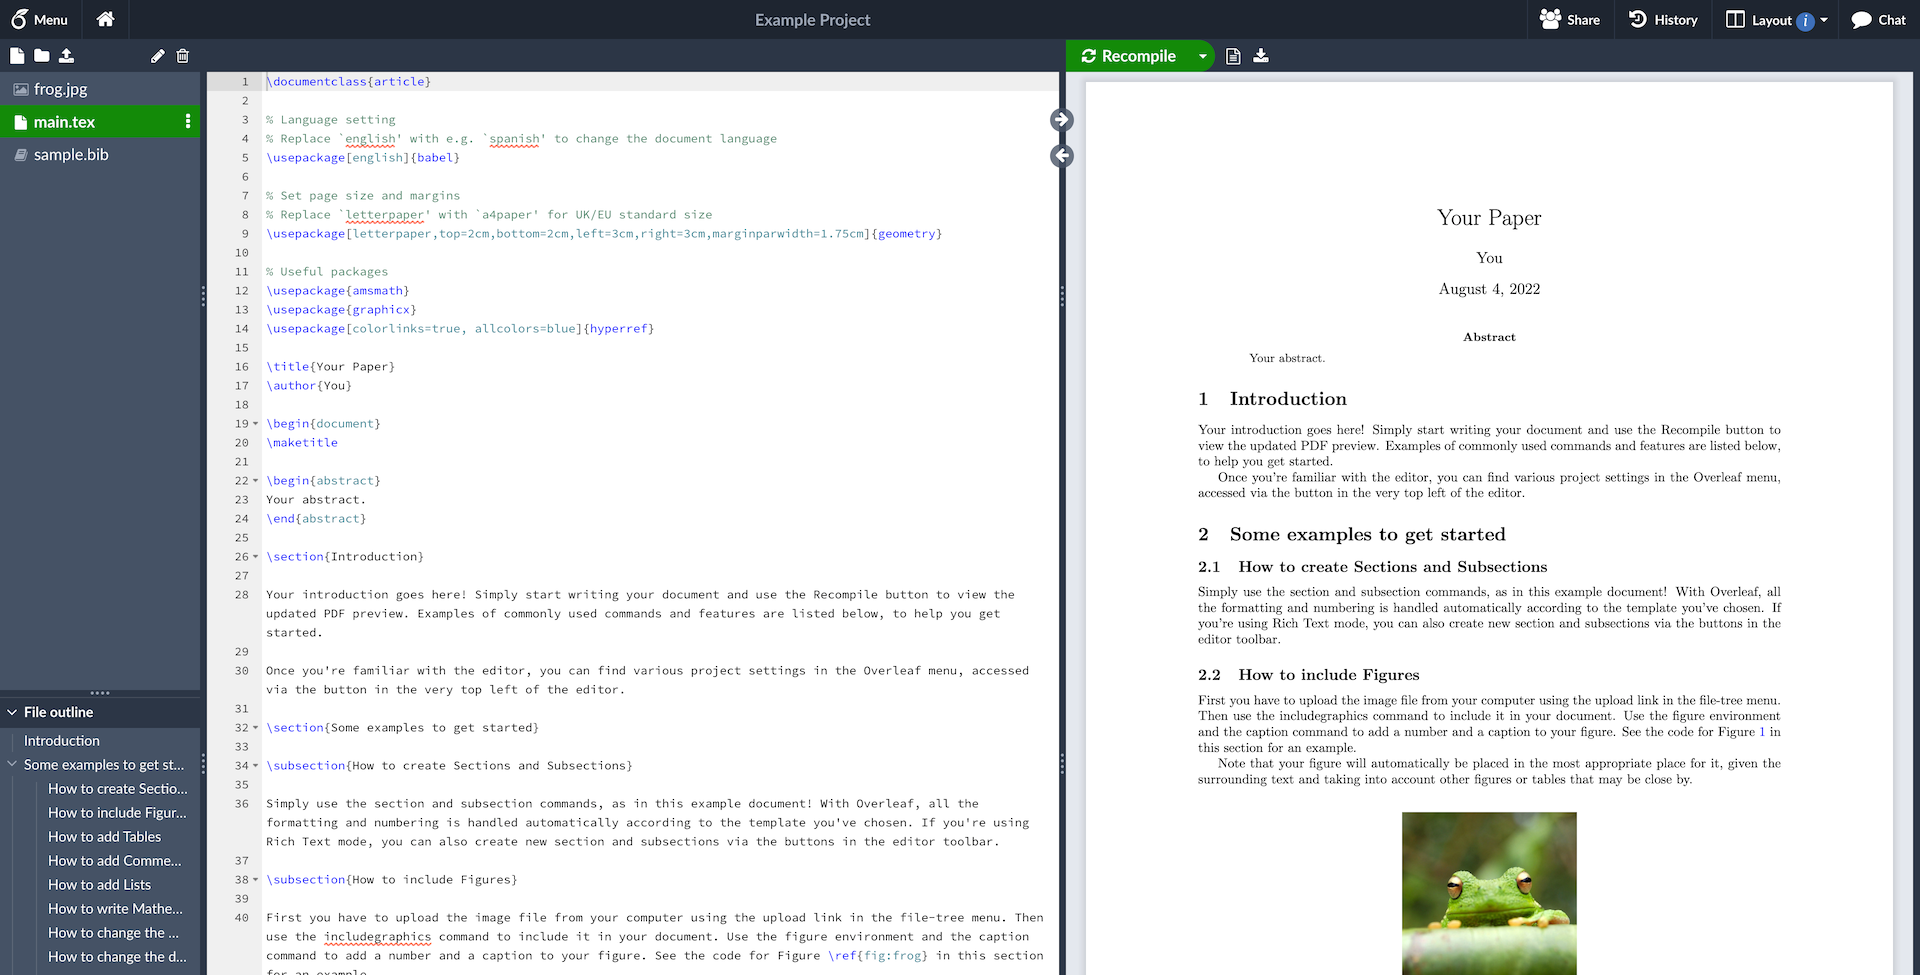
\includegraphics[width=0.85\textwidth]{img/overleaf.png}
  \caption{\centering{Overleaf editor. Source: \href{https://en.wikipedia.org/wiki/Overleaf}{wikipedia.org}}}
  \label{fig:overleaf_screenshot}
\end{figure}

\subsection{Versions}
\label{subsec:overleaf-versions}
Overleaf is available in three versions, which differ in features, levels of collaboration, deployment models, and costs.
Overleaf Community Edition (CE) is the free, self-hosted version designed for individual users and small teams. Overleaf Server Pro is the paid, self-hosted version tailored to organizations that offers advanced collaborative and administrative features. The cloud-based of Overleaf, instead, is offered as a service, comes in different tiers, and provides advanced features as well as various possibilities for integration.

\subsubsection{Overleaf Community Edition}
Overleaf CE\footnote{Overleaf Community Edition - \href{https://github.com/overleaf/overleaf/tree/main}{https://github.com/overleaf}} is free, open-source, and self-hosted. Although many collaborative features and integrations advertised by the company are not available in this version, it still represents an affordable solution for individual users and small research groups. Installation and setup are supported by the Overleaf Toolkit\footnote{Overleaf Toolkit - \href{https://github.com/overleaf/toolkit}{https://github.com/overleaf/toolkit}} and Docker, allowing users to deploy the software wherever they prefer. Beyond full control over data, privacy, and customization, this version has no restrictions on document compilation and supports unlimited collaborators per project. However, the company does not provide any support to the users, who have to rely on the community. 

\subsubsection{Overleaf Server Pro}
Overleaf Server Pro\footnote{Overleaf Server Pro - \href{https://www.overleaf.com/for/enterprises}{https://www.overleaf.com/for/enterprises}} is the self-hosted solution designed for organizations. It requires a paid license, which also guarantees priority support from the company. Compared to the CE, this version enables collaborative features, allows integration with Git, and provides a private template management system to share templates within the organization. Server Pro also supports SAML-based Single Sign On (SSO) and integrates some software optimizations.

\subsubsection{Overleaf}
Overleaf is the cloud-based solution for individual users, teams, and organizations. It is offered as a service and requires a paid subscription plan to access advanced features, but allows limited use with the free plan. Every paid plan enables all the collaboration features and allows integration with third-party services such as GitHub and Dropbox, as well as reference management software such as Mendeley and Zotero. In addition, they integrate Writefull, an AI-powered writing assistant, by default.
Groups and Commons tiers provide an advanced admin panel that, depending on the subscription, allows Single Sign On integration, automated user registration through LDAP or SAML, user account management and access to user metrics. Clearly, it doesn't require self-management of resources and guarantees automated updates and backups.
Since the free, standard, pro, and student plans are proposed for individuals, only Groups and Commons plans will be considered in this context and then unified as a unique solution.

\subsection{Hardware requirements and limitations}
Before diving into the sustainability assessment, it is necessary to clarify what specifications are required by self-hosted versions. Hardware requirements are published in the official GitHub wiki of Overleaf\footnote{Overleaf CE and Server Pro hardware requirements - \href{https://github.com/overleaf/overleaf/wiki/Hardware-Requirements}{https://github.com/overleaf}} and are shared between the two versions.
The minimal install requires 2 CPU cores and 3GB of RAM to support approximately 5 concurrent users. Then, it is suggested to add 1 CPU core and 1GB of memory for every 5/10 concurrent users. Therefore, the range provided by this rule is assumed to determine whether the allocation of resources is conservative (i.e. every 10 users) or aggressive (i.e. every 5 users). Allocating fewer or more resource could lead, respectively, to under-provisioning and over-provisioning.

With regard to storage allocation, Overleaf recommends using local disk storage for instances with fewer than 1000 users, which is approximately the limit suggested for the Community Edition. The maximum size allowed for a project is 500MB, but it is recommended not to exceed 100MB due to the size limit introduced by git integration. Considering that the size of the docker image is about 1GB and a full TeXLive installation is nearly 5GB, the storage requirement could be estimated as follows:
\[
\text{Storage}_{\text{exp}} = \text{Project size}_{\text{avg}} \times \text{Projects per user}_{\text{avg}} \times \text{Users}_{\text{exp}} \times \text{Backup space}
\]
For example, considering the base size, 25MB per project, 20 projects per user, and 300 users, while adding approximately 80\% of the space for backups, the required storage can be estimated at around 300GB.

The major constraint of Overleaf CE is that it supports only a single server deployment, meaning that all services, including the database, projects storage, and LaTeX compilation, must run on the same machine. This implies a severe limitation on scalability. In contrast, Overleaf Server Pro supports horizontal scaling, allowing multiple instances to share the workload through a load balancer and centralized storage. In this case, local storage is no longer supported and S3-compatible storage is recommended.

Table \ref{tab:overleaf_requirements} summarizes what has been discussed in this section, considering 300 expected users and 30 expected concurrent users.


\begin{table}[ht!]
    \centering
    % \small
    % \scriptsize
    % \tiny
    % \footnotesize
    \renewcommand{\arraystretch}{1.5} % Adjust row height
    \begin{tabular}{|>{\centering\arraybackslash}m{4cm}|>{\centering\arraybackslash}m{2.5cm}|>{\centering\arraybackslash}m{2.5cm}|>{\centering\arraybackslash}m{2.5cm}|>{\centering\arraybackslash}m{2.5cm}|}
        \hline
        \multirow{2}{*}{\textbf{Specification}} & \multicolumn{4}{c|}{\textbf{Overleaf provisioning - resource allocation}} \\
        \cline{2-5}
        & Under & Conservative & Aggressive & Over \\
        \hline
        Exp. number of Users & \multicolumn{4}{c|}{300}  \\
        \hline
        Exp. number of concurrent users & \multicolumn{4}{c|}{30} \\
        \hline
        Number of processors (or virtual processors) & 2 CPUs & 5 CPUs & 8 CPUs & 10 CPUs \\
        \hline
        Quantity of memory & 3 GB & 6 GB & 9GB & 12GB \\
        \hline
        Storage & \multicolumn{4}{c|}{300 GB} \\
        \hline
    \end{tabular}
    \caption{Overleaf hardware requirements for a large group of users}
    \label{tab:overleaf_requirements}
\end{table}

\section{Assessment of Overleaf through the sustainability framework}
\label{sec:4.2_overleaf_apply}
Universities aim to continuously improve academic productivity. In scientific departments and faculties, document production is often done with LaTeX, which offers better document control and scientific formatting compared to the traditional word processors. However, LaTeX comes with a steep learning curve, and its installation on user devices is not always fast and intuitive. Moreover, collaboration between users requires specific tools such as git or other version control systems, which require additional effort to become familiar with the workflow. In the context of digitization, this study assumes that the university would like to adopt a more efficient solution for the preparation of documents such as theses, articles, and publications by students, teachers, and researchers, particularly in scientific faculties.

Following the sustainability framework defined in the previous chapter, this section applies the methodology to Overleaf, evaluating its versions and whether they align with universities' needs and sustainability criteria. Each dimension is analyzed through its respective indicators. However, given the interconnections between certain indicators, some of them will be discussed together.
For each sustainability dimension, the results of the framework will be presented, providing an overview of Overleaf’s sustainability performance. A discussion and interpretation of the findings will be provided in the next chapter.

\bigskip

\subsection{Economic sustainability of Overleaf}
\label{subsec:overleaf-economic}
\medskip

\subsubsection{Return of expanses}
The return of expenses indicator analyzes the relationship between the cost of the DET and the value it generates. Overleaf has significant differences in costs among its versions, which are proportional to the number of features available. In the case of the Community Edition, the cost is determined by the amount of work required to install and configure the software, as well as the startup and maintenance of the hardware infrastructure. Apparently, this version could have a high initial return of expenses, which may decline as the number of users grows due to its limitations in scalability and administrative control. On the other hand, cloud-based and Server Pro versions are designed for enterprises and institutions, and the licensing (or subscription) costs are far from negligible. The generated value of these versions is nearly the same, with the self-hosted version potentially increasing cost efficiency as the number of users grows. However, the determining factor is the definition of generated revenue. For example, if the generated revenue is determined by rapid user adoption, the cloud-based may be preferred, while if the generated value is determined by control over the infrastructure, Server Pro may be preferred. Due to the difficulty of carrying out a systematic assessment, this indicator is not considered in the case study. 

\subsubsection{Provisioning and scaling policies}
The provisioning and scaling policies indicators evaluate, respectively, the cost of resources per user and the waste of resources. The technical characteristics of each version significantly impact resource management. Overleaf CE is limited to a single server machine, making scaling a critical factor and requiring accurate provisioning to avoid excessive costs. Server Pro instead supports horizontal scaling, enabling the distribution of computational load across multiple instances as needed. Meanwhile, the cloud-based version relies on a digital infrastructure shared among multiple users and organizations, ensuring optimal provisioning and efficient scaling. Clearly, the limited possibilities of the Community Edition are sufficient to assign a bad score, while the potential of Server Pro to reduce waste and increase cost efficiency in the long term justifies a good score. 

The assessment of this indicator is limited to a high-level perspective. A comprehensive study would require detailed knowledge of the infrastructure hosting Overleaf, as well as the associated and estimated costs of resource usage, which fall beyond the scope of this thesis.   

\subsubsection{Vendor lock-in and exit costs}
The vendor synergies and exit costs indicators evaluate the degree of dependency on the vendor’s ecosystem and the financial and technical effort required for migration. Regardless of the version, Overleaf is founded on standard LaTeX, which is an open-source technology. Therefore, it doesn't rely on proprietary formats or standards. Any project produced with Overleaf can be opened and modified with other LaTeX editors and can be compiled using other LaTeX distributions. In addition, users are allowed to export their projects at any time. In self-hosted versions, access to users projects is granted to the admins through their control dashboard, allowing mass export of projects inside the organization's workspace. 

Taking these factors into account, there is no evidence of vendor lock-in practices by the company in any version. However, some features may exercise a soft lock-in that does not affect the final outcome. For example, its ready-to-use nature and collaborative features may require users to make a considerable effort to gain expertise with local LaTeX distributions and familiarize themselves with alternative collaborative methods.

When migrating from Overleaf, the costs are determined only by the technical effort required for the digital infrastructure (if self-hosted) and for data export, which can be delegated to the individual users (except for the cloud version).

\bigskip

\subsection{Technical sustainability of Overleaf}
\label{subsec:overleaf-technical}
\medskip

\subsubsection{Availability and Reliability}
The availability and reliability indicators evaluate whether the software is operational and functions correctly. In the case of Overleaf, given its use for document production, its use is not confined to fixed times. Therefore, it must always be available. Furthermore, since it relies on the Internet connection, a high level of reliability is essential, particularly for content saving. However, compiler failures may rarely occur without significant consequences.

To assess the availability of Overleaf CE and the cloud-based version, both were monitored using Uptime Kuma\footnote{Uptime Kuma - \href{https://uptime.kuma.pet/}{https://uptime.kuma.pet}}, a popular self-hosted monitoring tool.
As shown in Figure \ref{fig:overleaf_availability}, the Community Edition instance maintained availability of nearly 100\% over a month. The cloud-based version showed the same result according to Uptime Kuma, which was also confirmed on the official status page\footnote{Overleaf Status Page - \href{https://status.overleaf.com/}{https://status.overleaf.com}}. 

\begin{figure}[ht!]
  \centering
  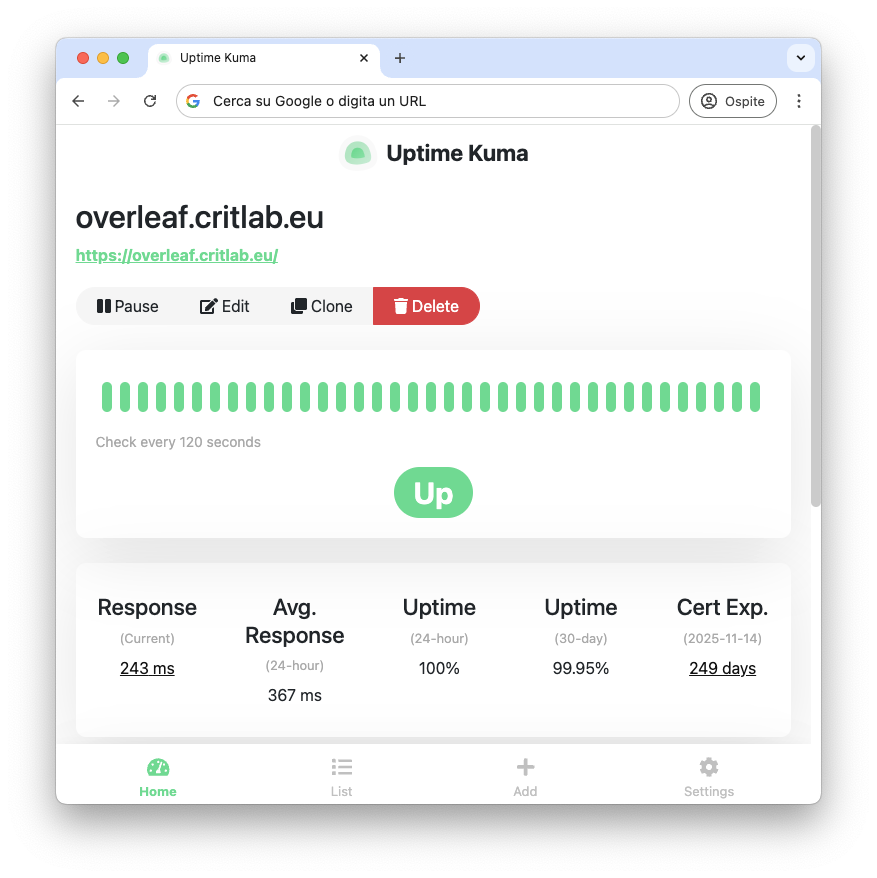
\includegraphics[width=0.6\textwidth]{img/overleaf_availability.png}
  \caption{\centering{Monitoring of Overleaf Community Edition with Uptime Kuma.}}
  \label{fig:overleaf_availability}
\end{figure}

To the best of the author's knowledge, Overleaf ensures reliability in all its versions, as confirmed for the cloud-based version by the incident history on its status page. 

\subsubsection{Scalability}
The scalability indicator assesses the ability of the system to meet changing demands. While for the cloud-based version this aspect is addressed by the service provider, the self-hosted versions support different levels of scalability that should be considered with respect to the underlying infrastructure. The Community Edition does not support any scalability techniques, thus the requirement is not satisfied. Instead, Server Pro supports load balancing and horizontal scaling, meeting the minimum requirement. Both versions support vertical scaling, but it will likely require manual intervention.

\subsubsection{Maintainability}
The maintainability indicator evaluates the ease of configuring, updating, and upgrading the software. As with the previous indicator, the cloud-based version is excluded, since the vendor is in charge of these operations. For Overleaf Community Edition and Server Pro, the level of maintainability is nearly the same, since they share tools and documentation. Before the introduction of Overleaf Toolkit, updates and upgrades were made through Docker images, and actually it is still possible to use this method. However, updates made by skipping some intermediate versions could lead to compatibility issues with dependencies. Now, these operations are performed through Overleaf Toolkit, which provides a useful script to simplify the process and limit the possibility of error.

The documentation is published in the official GitHub repository. It is not particularly complete, and sometimes appears hasty and informal, but it contains all the essential information. As for support, it is granted only to the Server Pro license owners, while for community edition users, support is delegated to the community.

Overall, the level of maintainability of both versions meets the minimum requirement, but the lack of direct support for the Community Edition should be considered. 

\subsubsection{Adaptability}
The adaptability indicator assesses whether the software supports integrations with university infrastructure and third-party services. Overleaf Community Edition does not support any built-in integrations with third-party tools. Overleaf Server Pro, however, supports Git integration and Single Sign-On, allowing user login to be integrated with the university administration system. In contrast, Overleaf Cloud provides several built-in integrations, such as Dropbox, GitHub, and reference management software. It also integrates generative AI for writing assistance.  

\subsubsection{Repairability}
The software repairability indicator evaluates whether the software and the underlying infrastructure allow interventions when issues and malfunctions occur. The key determining factors are the nature of the underlying infrastructure and whether the software is open-source or proprietary. Being open-source, Overleaf Community Edition, as well as Server Pro, allows interventions at both the code and infrastructure levels. If the software is not working properly, IT staff can take immediate action to resolve the issue and restore functionality. In contrast, the cloud-based version is fully managed by an external provider, preventing direct intervention and limiting the university's control in the event of malfunctions.

\bigskip

\subsection{Social sustainability of Overleaf}
\label{subsec:overleaf-social}
\medskip

\subsubsection{Community awareness}
The community awareness indicator assesses whether the service provider keeps the community up to date on changes and decisions that could affect the sustainability of the system. In this case, the indicator is applied uniformly across the three versions of Overleaf. The official Overleaf website has a blog section where the company publishes articles, news, and tutorials, but also changelogs, new feature announcements, and information about changes affecting the system. In addition to the infrequent publication of such information, it is evident that these updates are not driven by sustainability purposes, as this term is rarely or not mentioned at all.

\subsubsection{Involvement in sustainability}
The involvement in sustainability indicator measures the distance between the company and a sustainability claim. This indicator is evaluated by exploring the official website and searching for sustainability claims on the Web. The research was conducted by searching for related keywords such as "sustainability" and "environmental" along with other similar terms, in combination with "Overleaf" or organizations associated with it, as identified on the Overleaf website. Even though a more exhaustive investigation is necessary, this search did not produce any positive results. As a result, the company distance is more than one "hop".

\subsubsection{Inclusion}
The inclusion indicator states whether the software is compliant with accessibility standards. The evaluation was first conducted by searching for related keywords such as "accessibility" and "inclusion" in combination with "Overleaf" to find accessibility reports on the software. Then, compliance with WCAG was assessed using WAVE Evaluation Tool. Finally, although it is not aligned with WCAG, Google's Lighthouse tool in Google Chrome was used to confirm the findings of WAVE. Both tools were run in the editor view, with an empty project.

The results of the research show that no accessibility report is readily available. The evaluation with WAVE highlights the presence of many contrast errors and some missing alternative text for images, while other requirements, such as ARIA labels and structural elements, are fully compliant. Lighthouse, instead, identified some errors that did not align with WAVE's results. However, the tool provided three different scores for the same view, ranging from 65 to 85, and therefore its results are excluded from the evaluation.

Given the complexity of the software, it can be considered compliant with the minimum accessibility requirements.

\subsubsection{Privacy Policy}
The privacy policy indicator evaluates how users' data is collected and used. The assessment was first conducted by studying the privacy policy available on the official website, then identifying any sub-processors, and finally verifying the readability of the policy. 

Overleaf stipulates confidentiality contracts with third-party services and claims that user data may be shared with such services. However, many sub-processors are not explicitly mentioned in the privacy policy. Instead, they are listed on a separate page, which appears to be difficult to access within the website. Overleaf has numerous sub-processors, such as Google, Amazon, Heroku, Paypal, OpenAI, and many others (for the complete list, refer to Appendix \ref{cha:attachment_overleaf_comparison}).  Furthermore, information about the use of collected data by the integrated AI assistants, such as Writefull and TeXGPT, is displayed only while using the editor. Overleaf also uses analytics tools, such as Google Analytics.

The readability test was conducted using Readable\footnote{Readable - \href{https://readable.com/}{https://readable.com}}, Hemingway Editor\footnote{Hemingway Editor - \href{https://hemingwayapp.com/}{https://hemingwayapp.com}}, and GoodCalculators\footnote{GoodCalculators - \href{https://goodcalculators.com/}{https://goodcalculators.com}}, leading to the following results:
\begin{itemize}[noitemsep, topsep=4pt, parsep=0pt, partopsep=0pt]
    \item Flesch-Kincaid Grade Level: 12.7 (Readable), 13 (Hemingway Editor and GoodCalculators)
    \item Flesch Reading Ease: 39.7 (Readable), 35.4 (GoodCalculators)
    \item Gunning Fog Index: 14.6 (Hemingway Editor)
\end{itemize}
To obtain a good score, the Flesch-Kincaid Grade Level and Gunning Fog Index should be lower than 10, while Flesch reading ease score should be greater than 60. Thus, the cloud-based version does not satisfy the requirements of ethical approach and good readability, but it is compliant with the GDPR. 

The self-hosted versions, instead, are regulated by the university's own policy, since it is the only data processor. Clearly, if the university decides to integrate external analytics tools or to deploy the services to an external cloud infrastructure, then sub-processor are involved. Due to the total freedom in managing data processing, the self-hosted versions largely meet the requirements. 

\subsubsection{Capacity}
The capacity indicator evaluates whether the software is likely to generate internal capacity. The result is immediate because the cloud version is completely outsourced, while the self-hosted versions require skills and knowledge of deployment models, scaling techniques, and many other technical concepts. Given the higher complexity of Overleaf Server Pro compared to the Community Edition, the former requires more expertise than the latter. By the way, a significant factor to consider is that the self-hosted version is open-source and may encourage to contribute to the project. 

\bigskip

\subsection{Pedagogical sustainability of Overleaf}
\label{subsec:overleaf-pedagogical}
\medskip

\subsubsection{Engaged with instructional practices}
This indicator highlights whether the DET is founded on solid instructional practices or is actively involved in pedagogical research. As with previous indicators, the evaluation was first conducted by searching for related keywords, such as "pedagogical", "teaching", and "education" in combination with "Overleaf", to find evidence of the use of instructional practices or active research. Even if the research did not produce positive results, it was found that Overleaf is proposed as a digital education technology. The focus, aside from research, is on teaching, since the company claims that its features, such as documentation and presentation production, as well as template sharing, can improve the teaching experience. Anyway, these features were not specifically designed for teaching, but to increase writing productivity, especially for researchers.

\subsubsection{Usability}
The usability indicator verifies how efficient and user-friendly a digital technology is. The evaluation was conducted by reviewing the criteria described in Section \ref{sec:3.1_framework_structure}. Since Overleaf is focused on LaTeX, which has a significant learning curve, an important aspect is how the editor simplifies its use. A summary of the factors considered is presented in the following list:
\begin{itemize}[noitemsep, topsep=4pt, parsep=0pt, partopsep=0pt]
    \item Learnability - Overleaf provides a comprehensive and free-to-access LaTeX documentation, as well as tutorials for Overleaf and crash courses. Basic tasks such as simple text formatting (e.g., italic, bold, lists) and insertion of hyperlinks, tables, and formulas can be done with the toolbar, allowing users to familiarize themselves with the editor.
    \item Efficiency of use - Overleaf provides a comprehensive list of hotkeys for common tasks. In addition, it also provides auto-complete features for commands, images, references, and many other elements. The editor offers a split-screen view with the project navigator and the output file preview on the sides.
    \item Error prevention and user control - Overleaf identifies some errors (e.g. unclosed commands) before compilation. Otherwise the compiler will list the errors, which unfortunately are often not self explaining. The toolbar and the hotkeys help to prevent writing errors.
    \item Feedback and transparency - Typically, when the software faces an issue, such as connection errors or rendering errors, it displays a message to the users. However, sometimes it does not provide any feedback, making it difficult to understand the state of the system (e.g., it is assumed that the software is connected because there are no error messages).   
    \item Integrations and customization - Integrations are available only in paid versions, and the cloud version supports more integrations than Overleaf Server Pro. Overleaf allows basic customization such as font family, font size, line height, and editor theme. Other customizations relate to auto-completion and compiler configuration.
\end{itemize}
Considering that environmental setup is no longer necessary, Overleaf meets the requirements, but a more detailed assessment would be necessary. 

\subsubsection{Purpose and Impact on education}
The purpose and impact on education indicators cannot be evaluated in a purely systematic way, but should be discussed to obtain a better picture of the problem. Purpose refers to the motivations that lead to the adoption of a technology, while impact on education tries to understand what are the implications of this adoption.

In this study, it is assumed that the university wants to adopt Overleaf to improve document preparation for students, teachers, and researchers. In scientific faculties, LaTeX is widely used for many purposes, and the introduction of Overleaf in the existing workflow would bring several benefits, such as greater collaboration, less complexity in setup and configuration, and many others. For example, a student who is preparing his final dissertation can easily share the project with its supervisor, who can check the content and suggest changes through the review feature. If the previous workflow is based on local LaTeX, these operations were probably done via e-mail, and this clearly represents an improvement. Another example: a group of researchers that is preparing an article can easily share the project among the team members, ensuring that they work always on the latest version. These use cases validate both the purpose and the impact on education.

But what if the university wanted to adopt Overleaf for word processing? Clearly, this scenario is the completely opposite of the previous one, adding unnecessary complexity, requiring additional effort, and probably disrupting the existing workflow. The steep learning curve and required skills would lead to a negative impact on education. Overleaf is not suitable for everyone; it has a strong orientation toward STEM disciplines, and this must be carefully considered when evaluating its adoption.

To conclude, based on the assumption, Overleaf can improve document preparation within the institution, and its impact on education is positive.

\bigskip

\subsection{Environmental sustainability of Overleaf}
\label{subsec:overleaf-environmental}
\medskip

\subsubsection{Energy and raw material consumption, carbon emissions}
These indicators estimate the environmental impact of the technology under examination. To find an environmental assessment about Overleaf, a search was conducted using related keywords such as "environmental", "assessment", "emissions", and "energy" in combination with "Overleaf". Unfortunately, the research did not produce any result, but some considerations can be inferred by looking at Overleaf's sub-processors.

Overleaf declares that it relies on Amazon AWS, Google Cloud Platform, Heroku and MongoDB Atlas for hosting. As discussed in Chapter \ref{cha:2_dets-and-sustainability}, the relationship between Big Tech companies and the environmental impact is far from trivial. Large data centers continue to rely on energy produced from fossil fuels due to their low cost and widespread availability. To meet renewable energy requirements, companies often rely on renewable energy certificates (RECs) \cite{khosravi_review_2024}\cite{stacey_pollution_2025}. Through RECs, companies claim to produce, elsewhere or in-site, an equivalent amount of renewable energy compared to the energy used by the data centers. However, this practice does not ensure that the data centers are actrually supplied by renewable energy, and RECs have been criticized for allowing companies to claim zero-emissions or low-impact status without substantial proof. Considering their low willingness to share data on environmental impact, the lack of transparency, and contribution to e-waste generation, software relying on big cloud providers cannot get a good score with these indicators.

For on-premises solutions, instead, the indicators are not applicable due to the lack of knowledge about the system that will host the software. Nonetheless, a neutral score is assigned because of the potential to rely on environmentally responsible infrastructures. 

\subsubsection{Sustainability in design and through design}
The sustainability in design indicator states how sustainability is considered as a software quality, while the sustainability through design indicator evaluates the impact the technology has on users. As shown in the assessment of community awareness indicator, there is no evidence that sustainability concerns were accounted for in the design phase. Moreover, some considerations can be done simply by using the software. First, the editor pushes users to compile frequently due to its association with the typical saving mechanism, which increases the computational load and related energy consumption. Then, the real-time collaboration feature requires a persistent connection to synchronize data. Finally, it is not clear whether the company uses a less efficient algorithm or fewer computational resources for free or cheaper plans. Deploying a self-hosted version to a sustainable infrastructure can mitigate these issues, but cannot solve them.

Regarding sustainability through design, the outcome is nearly the same. For example, the user interface does not show the user any information about resource usage. As another example, the software does not support any low-power or energy saving mode and users are not able to customize the software to significantly reduce its resource usage. To the best of the author's knowledge, Overleaf does not encourage sustainable practices through its software.

\section{Result}
\label{sec:4.3_overleaf_result}
The overall result of the assessment is shown in Figure \ref{fig:overleaf_result_overview}. Every row represents one of the 25 indicators within its dimension, while each column represents a version of Overleaf. As described in chapter \ref{cha:3_framework}, each color is associated with a score, where green is 1, yellow is 0, red is -1, and gray means not applicable. The final score is displayed at the bottom and is shown in relation to the number of indicators applied. 

\begin{figure}[ht!]
    \centering
    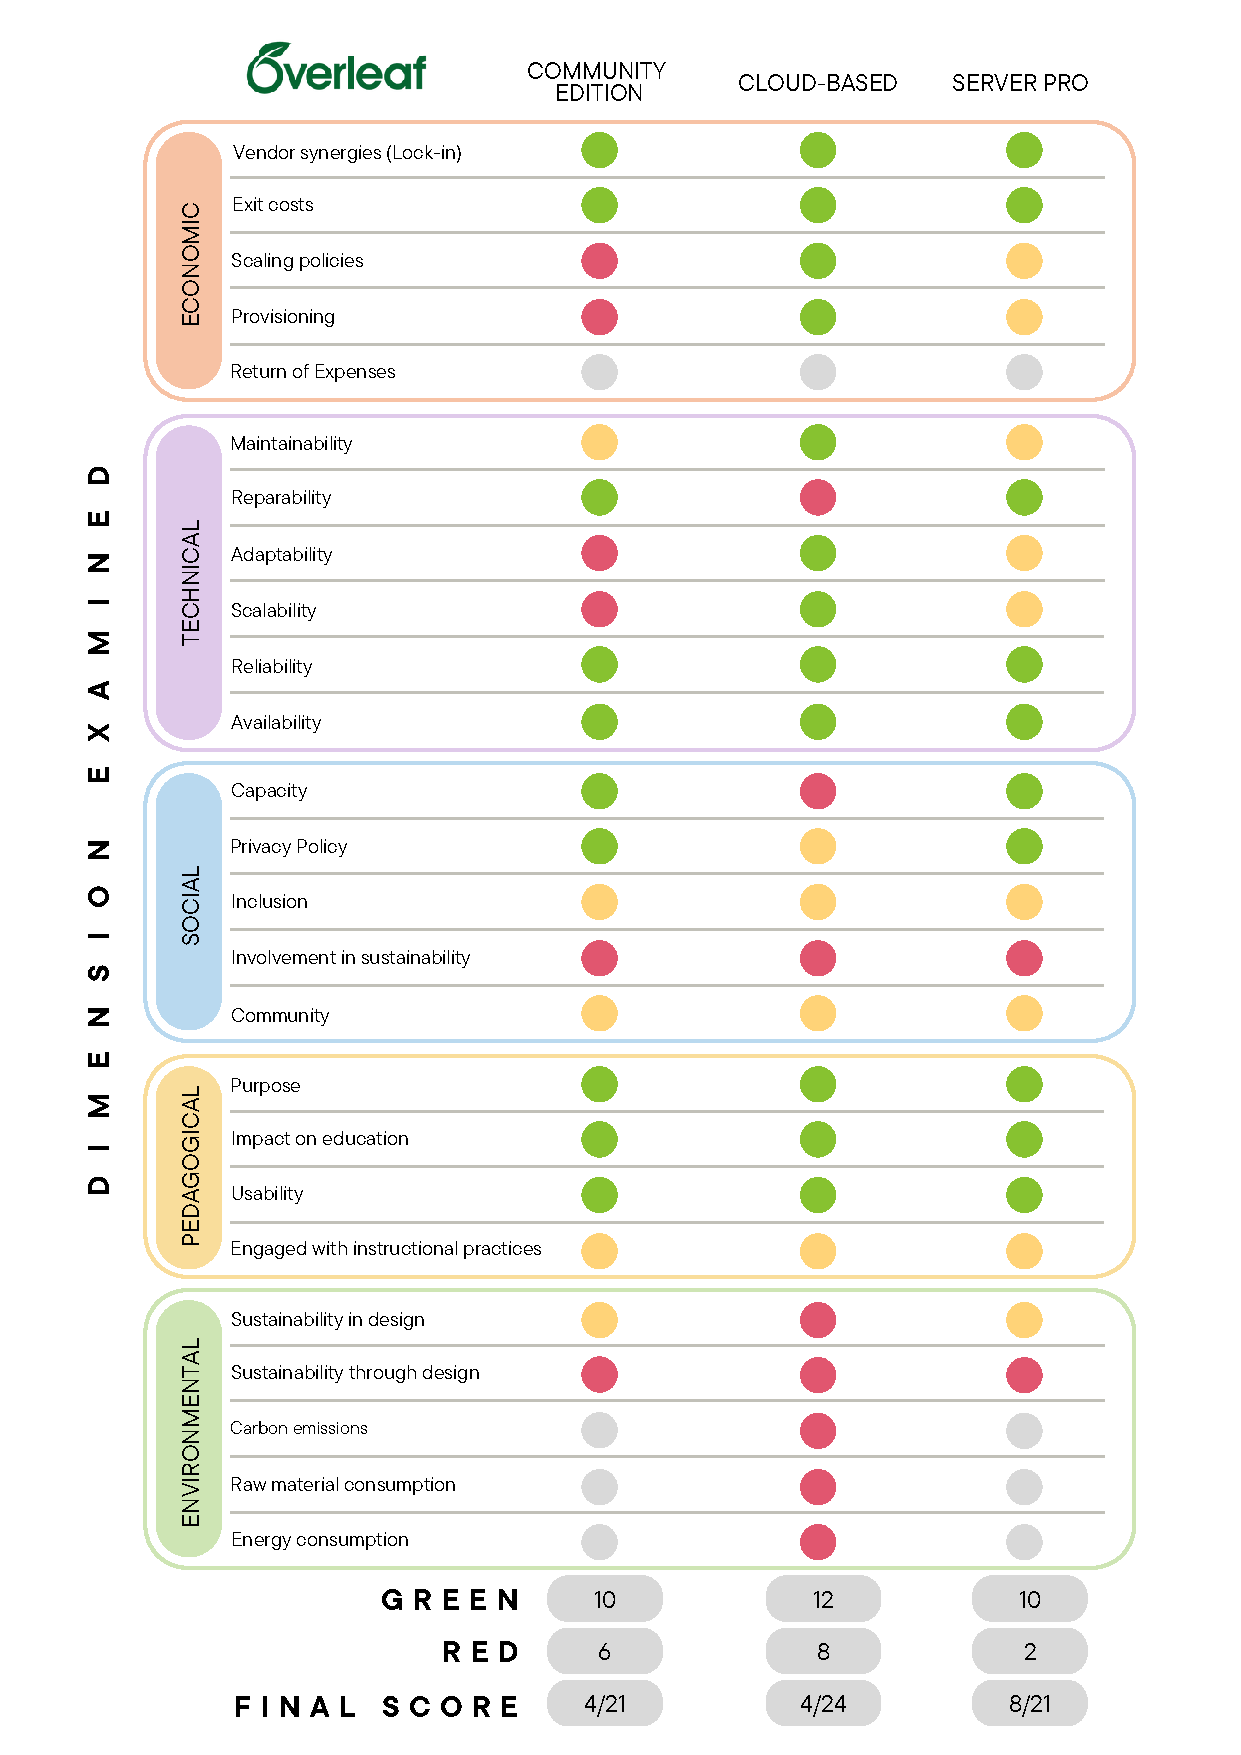
\includegraphics[width=1\textwidth]{attachments/overleaf_result_overview.pdf}
    \caption{Overall result of Overleaf's assessment}
    \label{fig:overleaf_result_overview}
\end{figure}

% ATTENZIONE aggiungere score verde e score rosso allo schema
% trattare l'argomento nelle conclusioni
% magari insieme alla parte sulle zone rosse

% PER PRESENTAZIONE: qual è il messaggio principale????
      \newpage
      \ % The empty page
      \newpage
      
      \chapter{Discussion}
\label{cha:5_discussion}
This chapter discusses the overall results of the assessment, focusing on how the sustainability framework performed and highlighting critical aspects found in the process.     

\section{Summary of the results}
\label{sec:summary_result}
Based on the results shown in Figure \ref{fig:overleaf_result_overview}, the Community Edition scored 4/21, the cloud-based version 4/24, and the Server Pro version 8/21. Overleaf Server Pro achieved the most balanced score across all evaluated dimensions, except for the environmental dimension, which suffers from the non-applicability of many indicators. As expected, the cloud-based version performed best in the economic and technical dimensions, reflecting the reasons why universities often rely on external cloud infrastructures for their services. On the other hand, the Community Edition obtained a low score due to technical shortcomings, which were predictable given its focus on individual users and relatively small work groups.

A key finding, highlighted by the traffic light system, is that when considering equivalent core functionalities, the way the software is deployed does not affect its pedagogical quality. This means that regardless of the chosen version, the impact on the educational experience remains the same. Consequently, once the pedagogical validity of the technology is established, the other dimensions become decisive in determining which version should be preferred. In contrast, the way the software is deployed may affect the social dimension, as cloud-based solutions do not require technical expertise from institutions, and policies applied by providers tend to collect user data intensively.

Another important insight emerging from the results is that when a university relies on its own infrastructure and internal expertise instead of private providers, it can mitigate many of the challenges associated with using external services. For example, in the environmental dimension, the university has almost full control, allowing it to decide on the type of infrastructure to use, the energy sources to rely on, and the implementation of techniques to minimize its environmental impact. The same applies to the social dimension, where the university gains greater control over data and its management. Consequently, the only remaining limitations are the technical qualities of the education technology itself, which are inherently tied to how the technology was developed and represent one of the few factors beyond the institution’s full control.

\section{Scoring system and weight of indicators}
The framework was designed by assigning equal weight to each indicator. This ensures fairness among the developed indicators, but implies that the number of indicators assigned to a specific dimension determines its overall weight. For example, in the cases of Overleaf Community Edition and Server Pro, the non-applicability of the indicators related to the environmental impact of energy and material consumption reduces the influence of the environmental dimension on the final score. This shift lowers its potential impact from \(\pm\)\ 5 points to approximately \(\pm\)\ 2 points. The same principle applies to other dimensions with fewer indicators or in cases where, at the discretion of those in charge of the assessment, an indicator is re-assessed in a different dimension.

This misalignment with the core principles of the framework must be considered, as each dimension is intended to be equally important in assessing sustainability. A future revision of the framework could consider to re-balance the weight of each indicator based on the quantity of indicators within each dimension. This adjustment would ensure that every dimension can influence the final outcome equitably, whether positively or negatively.

Finally, another aspect to consider regarding the scoring system is that, despite the Server Pro version receiving positive evaluations across most of the indicators, its final score remains surprisingly low. This raises some concerns about the point allocation mechanism, which appears to be overly strict. However, certain aspects of sustainability cannot be overlooked.

\section{Dealing with red zones}
A crucial question that arises from the overall results concerns how to deal with "red zones”:
\begin{center}
    \textit{“What actions should be taken if none of the indicators within a given dimension meets the minimum sustainability criteria?”}
\end{center}

As discussed in the literature review in Chapter \ref{cha:2_dets-and-sustainability}, if a sustainability dimension is overlooked, other dimensions will also be affected. This interdependence is evident in the case of Overleaf cloud-based version, where the weaknesses in the environmental dimension negatively impact the social dimension. Specifically, the lack of transparency about the underlying infrastructure and its impact leads to the neglect of the community and its involvement. Similarly, as observed in the results for Overleaf Community Edition, technical limitations affect the economic dimension. Nevertheless, if none of the indicators within a single dimension achieve a positive evaluation, this should be considered a sufficient criterion for excluding the technology from the selection process.

\section{Challenges of multi-dimensionality and limitations}
%As with any research, the results and implications of this study have to be considered within the context of the research limitations. 
The most significant limitation of this study is its multi-dimensionality, which arises from the nature of sustainability and introduces various challenges both in defining the criteria to be considered and in the evaluation process itself. The application of the framework has proven to be a complex and interdisciplinary process, which risks emphasizing the lack of knowledge in disciplines outside the area of those in charge of the process. For this reason, in this study, the evaluation of many indicators was conducted from a high-level perspective.

Huang M., in his research on DET selection processes \cite{huang_building_2023-1}, demonstrates that in some European universities, this process involves a broader working group, ensuring greater expertise across all relevant disciplines.
Moreover, the case study of this thesis represents only one of many possible scenarios. This selection process is often triggered not only when there is an intention to adopt a new technology, but also when it becomes necessary to replace an existing one. While the framework has performed as expected, further case studies are needed to assess its effectiveness comprehensively.

      \newpage
      
      \chapter{Conclusion}
\label{cha:6_conclusion}
The digitalization of universities continues to evolve rapidly, raising concerns about how sustainability is integrated into this process. The selection of education technologies remains an area with little critical attention, highlighting the need for further research to ensure more informed and sustainable choices. This thesis addressed the issue by first defining the sustainability dimensions for digital education technologies and then proposing an evaluation model to be used in the selection process.

\section{Key insights}
The most important findings in the assessment are resumed as follows:
\begin{itemize}[noitemsep, topsep=4pt, parsep=0pt, partopsep=0pt]
    \item The results confirm that the sustainability in digital education technologies is a multi-dimensional issue that extends beyond mere economic considerations. While financial constraints remain a primary factor in technology procurement, institutions must integrate other sustainability dimensions into their decision-making processes. A structured framework, such as the one developed in this study, enables universities to make more informed choices.
    \item The assessment confirms that the way the software is deployed (cloud-based, self-hosted) does not impact pedagogical effectiveness. Once a technology meets the required educational criteria, other factors such as economic, environmental, and social sustainability become the decisive elements in its selection.
    \item Self-hosted solutions provide improved data governance and more control over environmental impact. However, they remain subject to external technical constraints, such as software architecture and update cycles, which may impact their sustainability in the long-term.
    \item The evaluation confirmed the interconnected nature of the sustainability dimensions, as weaknesses in one sustainability dimension can negatively affect others.
\end{itemize}

\section{Future works}
This study, as discussed in the previous chapter, is not without limitations and presents several opportunities for future research and refinement. 

One of the key areas for further development is the application of the proposed framework to a wider range of case studies. While it has been tested on a specific technology, its adaptability to other digital education technologies and different institutional contexts remains to be explored. As an example, applying the framework to case studies involving DET migration, where institutions transition from one system to another, would provide valuable insights into its practical utility and robustness. Once the framework is validated theoretically, it should be implemented in real-world selection processes to assess its effectiveness in guiding decision-making.

Another crucial aspect is the set of indicators used for evaluation. The indicators in this study were derived from the current state of research, meaning they are not exhaustive and could be expanded as the field evolves. During the framework's development, some indicators were discarded due to challenges in their applicability or measurement, such as resistance to decay and network effects. Future research could revisit these aspects, determining whether they hold value in specific contexts or whether alternative indicators could better capture relevant sustainability factors.

In addition, there is a significant opportunity for improvement in the development of metrics, particularly within the environmental dimension. The complexity of assessing the environmental impact of DETs remains a challenge, as many existing methodologies require extensive data collection and analysis, making them difficult to implement in practice. To address this, more intuitive and comparable metrics should be explored. For example, impact labels, similar to energy efficiency labels used for household appliances, could simplify the assessment of the environmental footprint of digital technologies. Easier sustainability assessments could enhance the framework’s accessibility and usability, supporting more informed decision-making in technology selection.

Future research should also investigate ways to improve the scoring system and indicator weighting to ensure that all dimensions of sustainability are equally represented. As noted in the discussion, certain aspects may currently be under weighted or overemphasized, potentially leading to an imbalanced evaluation of DETs.

Ultimately, this study lays the groundwork for a multi-dimensional assessment of sustainability in digital education technologies, but its full potential can only be realized through further validation, refinement, and practical application.


      \newpage
      
    \endgroup


    % bibliography - bibtex format
    %
    % add chapter to index
    \addcontentsline{toc}{chapter}{Bibliography}
    % alphabetical order of authors
    \bibliographystyle{plain}
    \bibliography{bib/bibliography}
    
    \newpage
    \ % The empty page
    \newpage

%% Note
%% In the bibliography, all the sources consulted for the dissertation 
%% have to be cited and listed in alphabetical order by the 
%% first author's surname.
%%
%% According to the source material, the quotation has to be as follows:
%%
%% BOOKS
%% Surname and initial/s of the name/s of the author/s, date of edition,
%% publishing house and (if applicable) number of edition.
%% 
%% JOURNAL ARTICLES 
%% Surname and initial/s of the first name/s of the author/s,
%% title of the article, name of the journal, volume number, issue number
%% and page numbers.
%% 
%% CONFERENCE PAPERS
%% Surname and initial/s of the name/s of the author/s,
%% year of the conference, title of the article, name of the conference,
%% place of the conference, conference dates, page numbers.
%% 
%% CITING WEB RESOURCES
%% The consulted webpages have to be listed in alphabetical order. 
%% It is necessary to:
%%   - Copy the specific URL (the web address) of the consulted webpage
%%   - If available, indicate the surname and first name of the author/s,
%%     the title and subtitle of the text
%%   - If available, indicate the last date you retrieved the webpage
%%     (day/month/year).   

    \titleformat{\chapter}
        {\normalfont\Huge\bfseries}{Appendix \thechapter}{1em}{}
    % Appendix / attachment section - optional
    \appendix
    % \chapter{Indicators overview}

\chapter{Supporting Documents}
\label{cha:attachment_overleaf_comparison}

\section{Overview of Indicators}
Figure \ref{fig:A1_attach_indicators_overview} provides an overview of the indicators defined in Chapter 3. In the figure, the indicators are accompanied by their dimensions, metrics, and results assignment criteria.

\section{Comparison between Overleaf versions}
Figure \ref{fig:A2_attach_overleaf_overview} presents a detailed comparison table of the different versions of Overleaf. The table includes features, integrations, and administration capabilities. Additionally, it provides the minimum installation requirements and a categorized list of sub-processors. For completeness, the pricing of the various plans is also included.

\newpage

% DIGITALE SENZA NUMERO
% 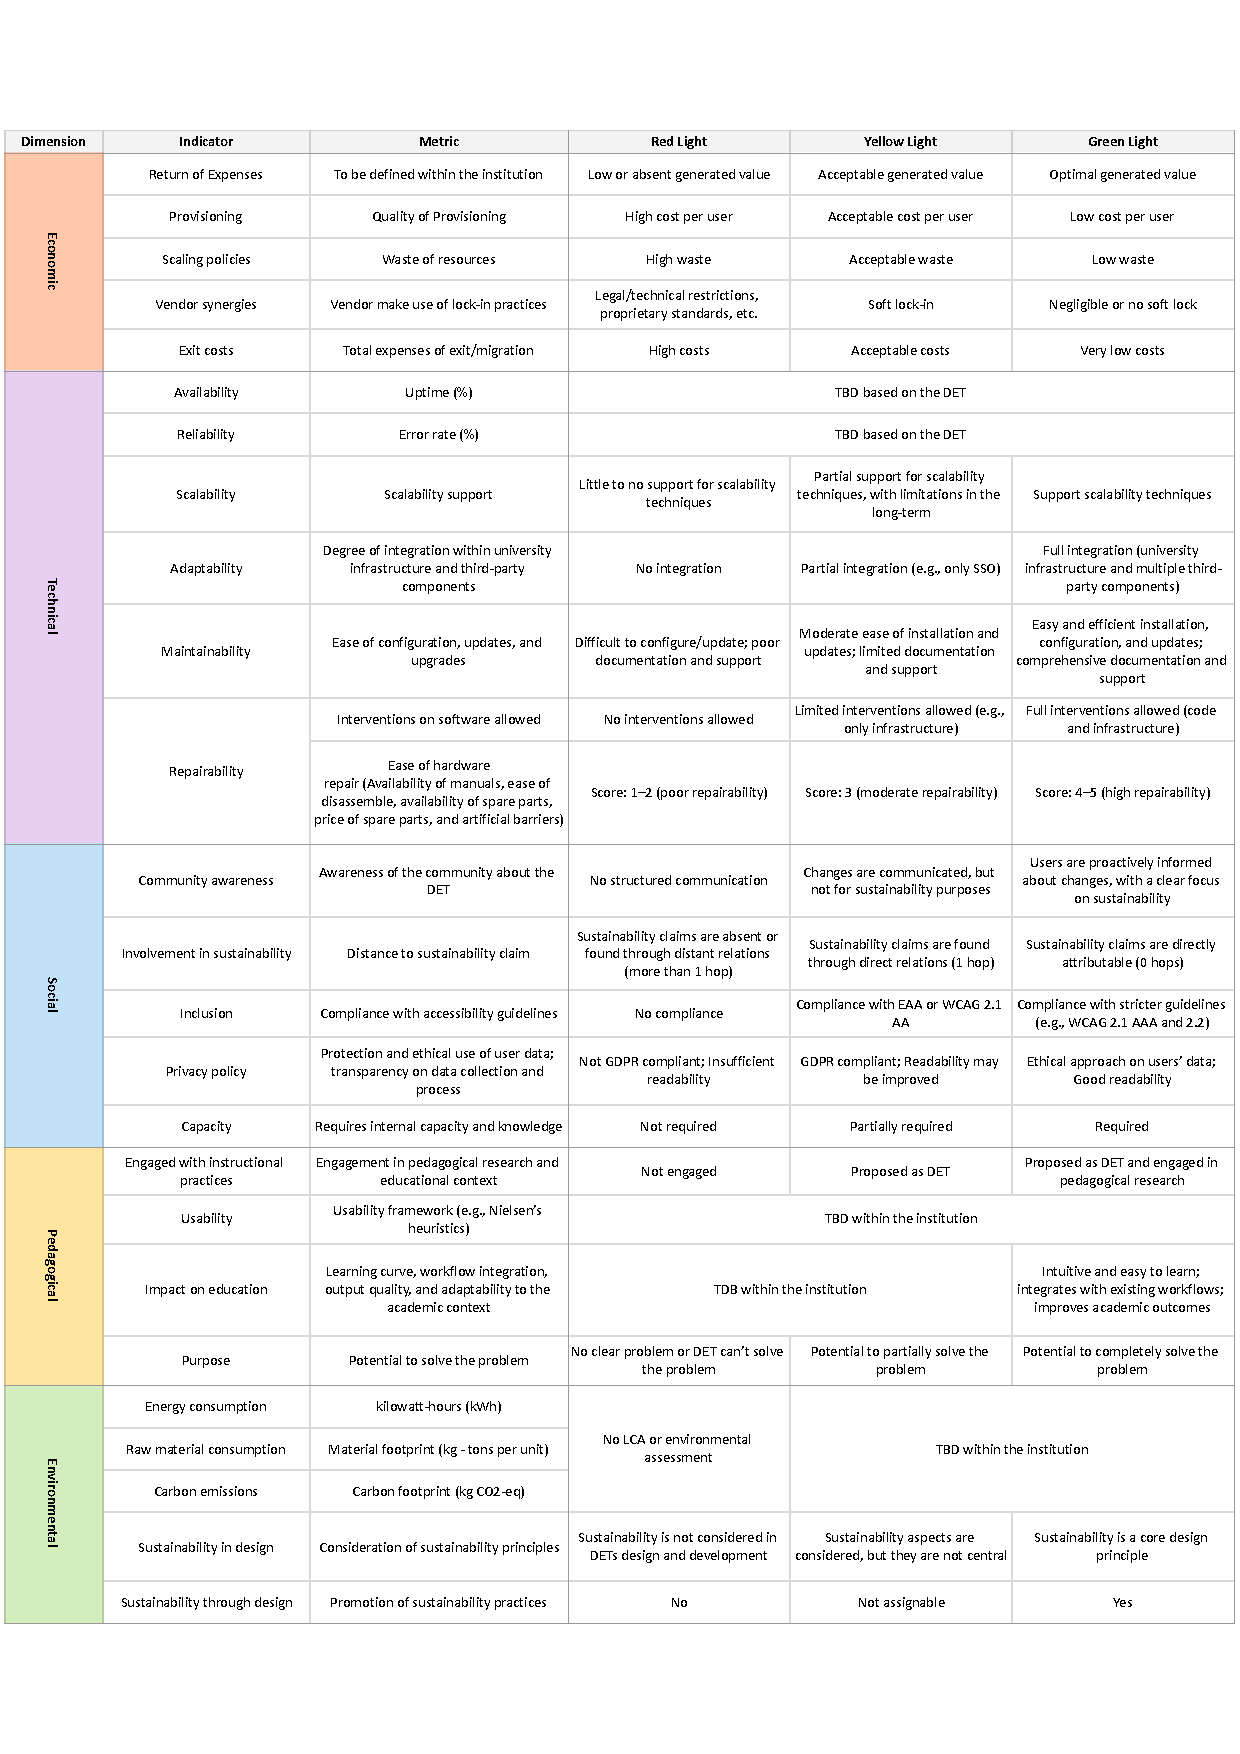
\includepdf[pages=1, fitpaper=true]{attachments/indicators_overview.pdf}
% 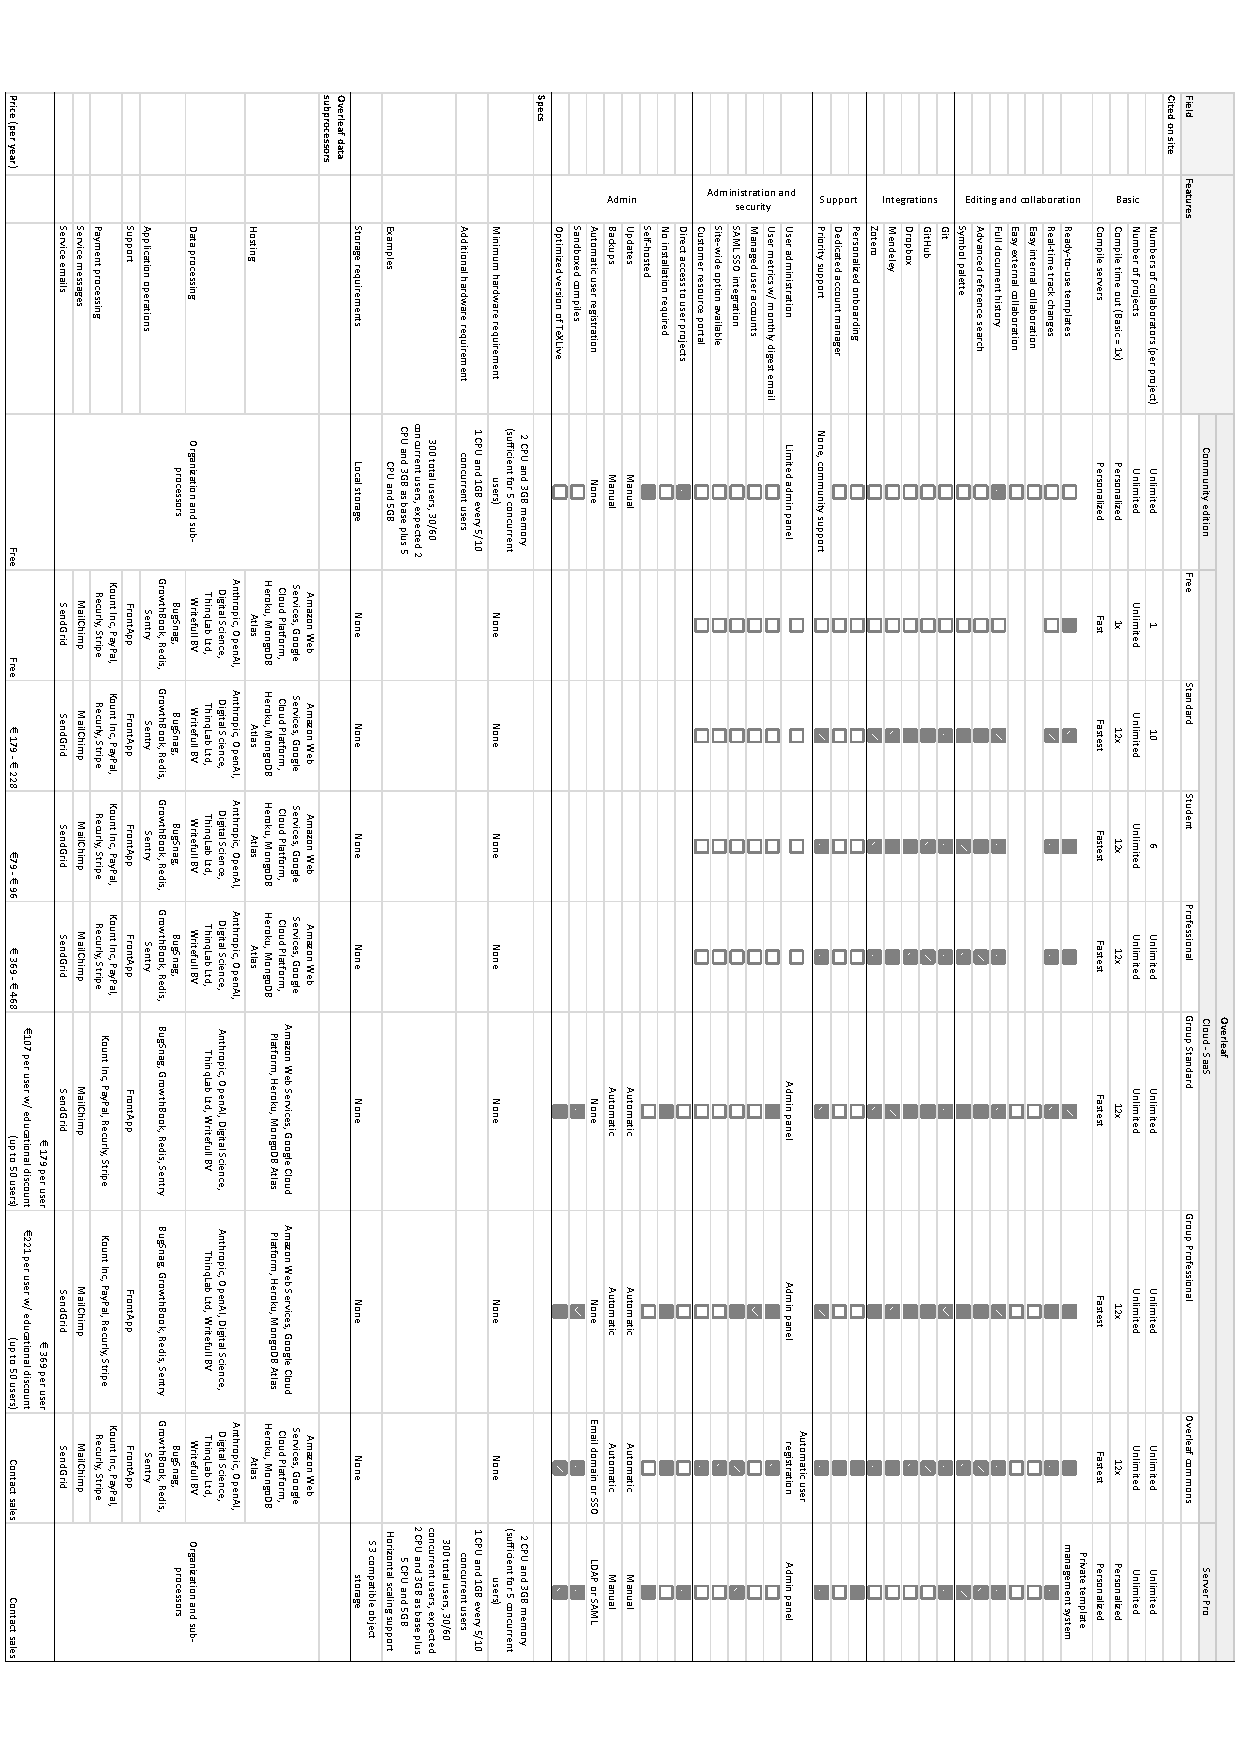
\includepdf[pages=1, fitpaper=true]{attachments/overleaf_overview.pdf}

% DIGITALE CON NUMERO
% \begin{figure}[ht]
%     \centering
%     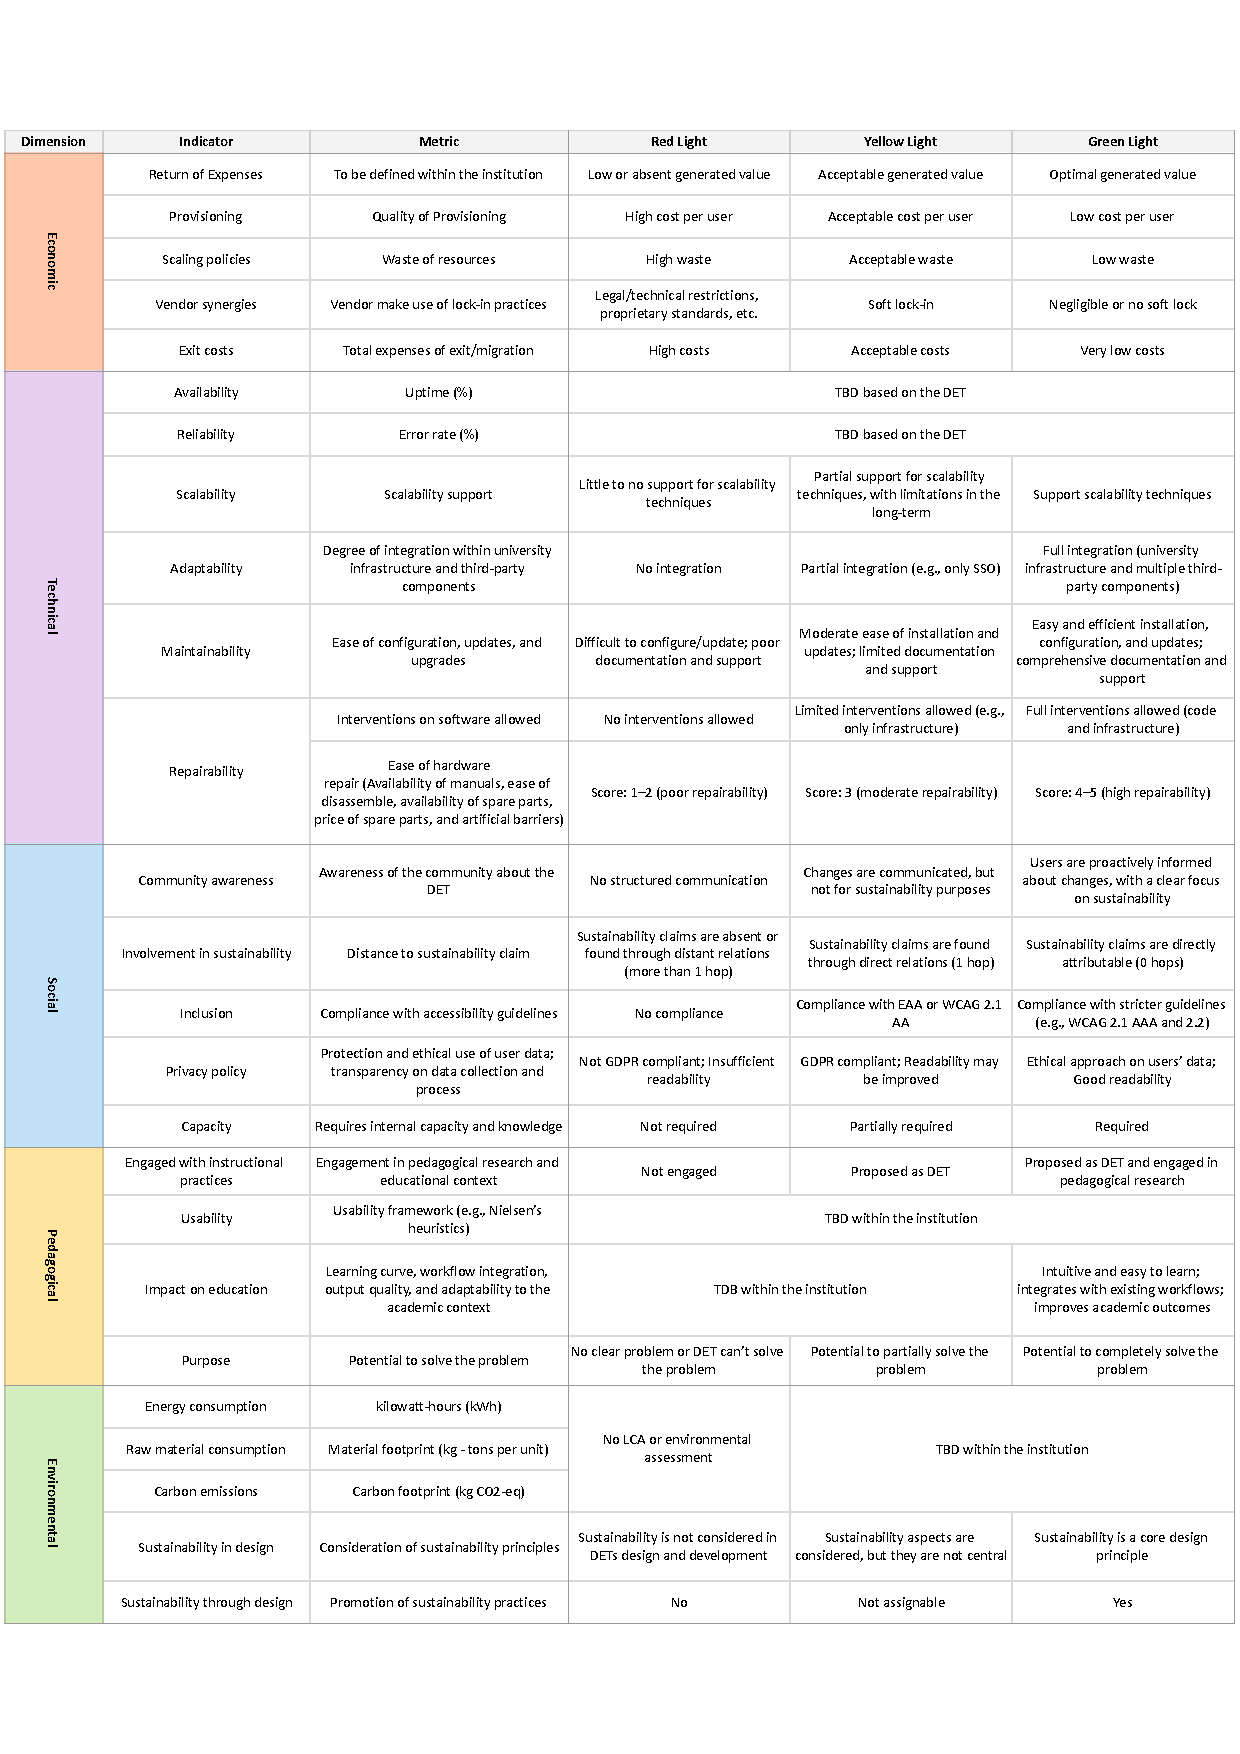
\includepdf[pages=1, scale=0.8]{attachments/indicators_overview.pdf}
%     \caption{Overview of indicators}
% \end{figure}

% \begin{figure}[ht]
%     \centering
%     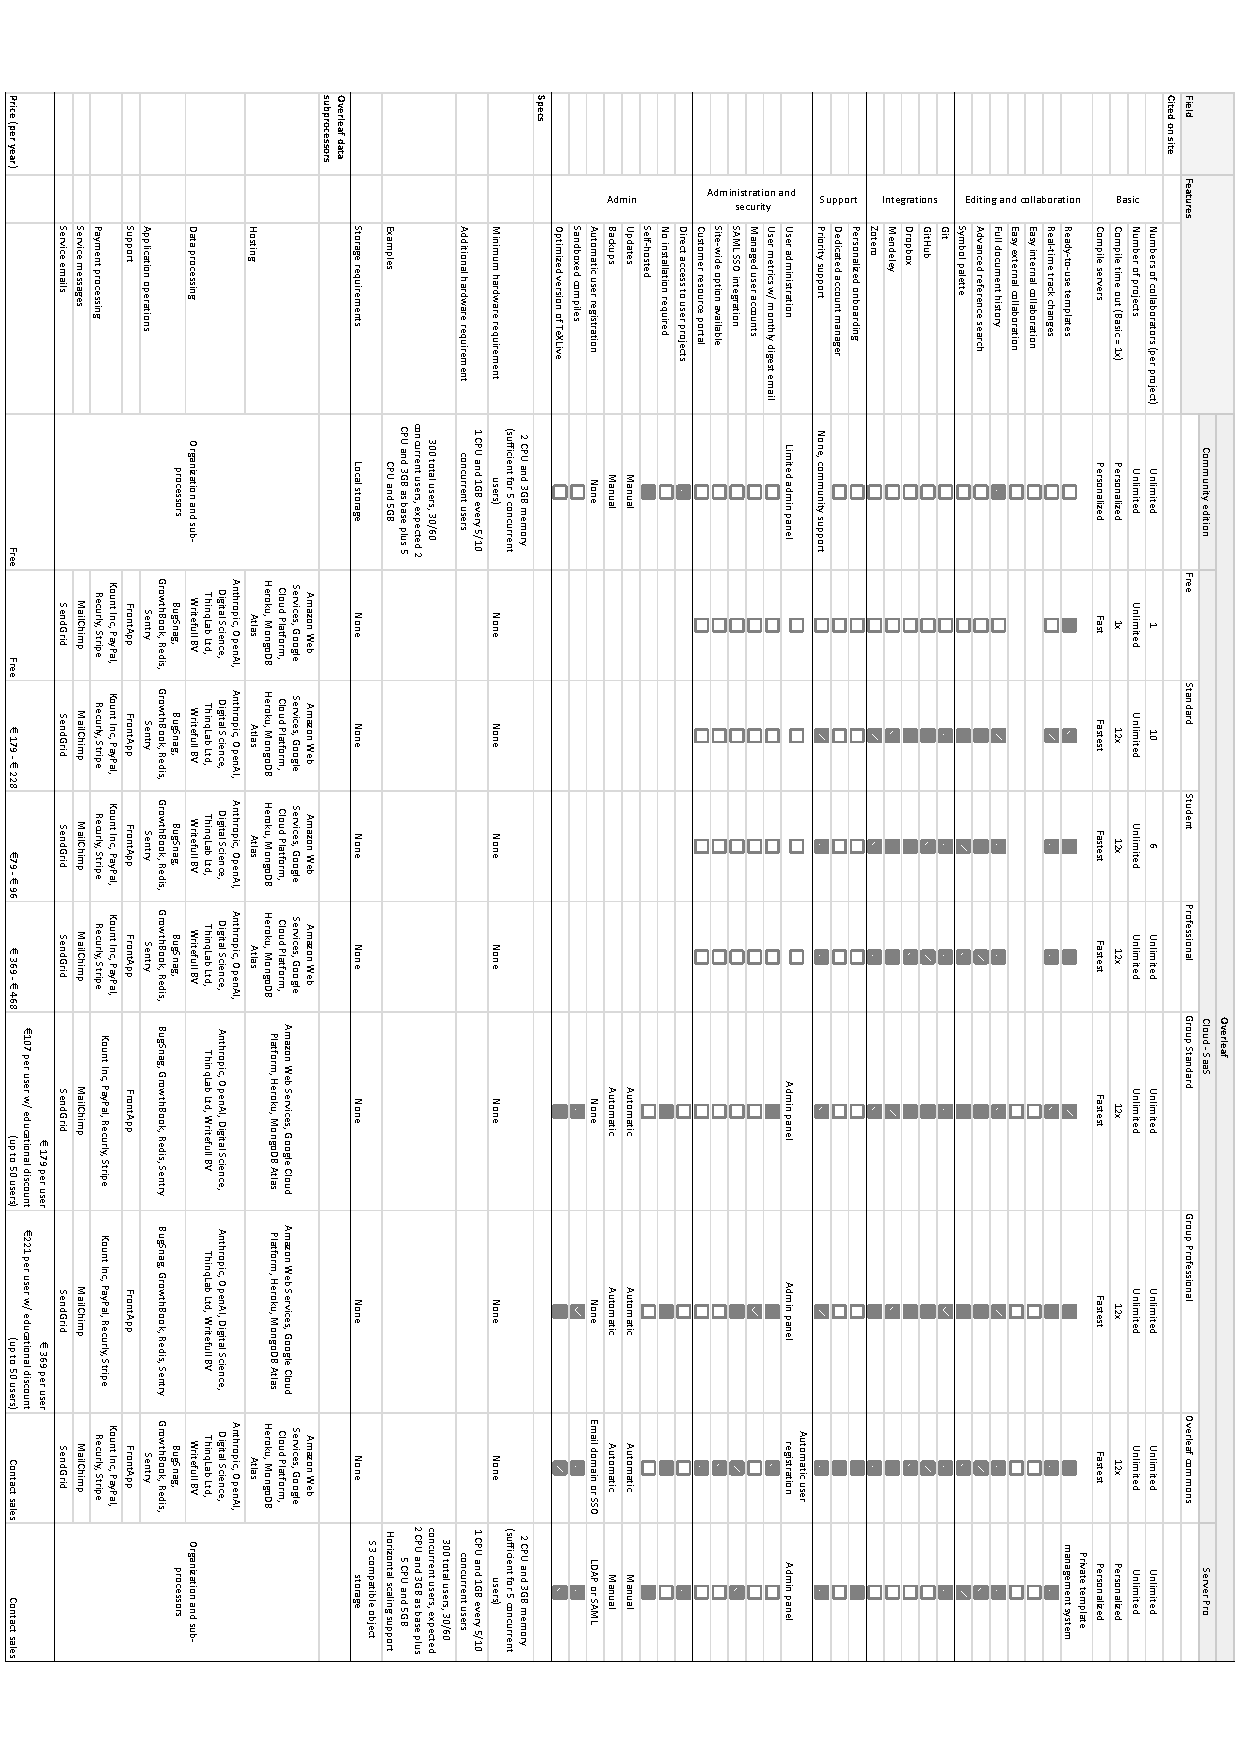
\includepdf[pages=1, scale=0.8]{attachments/overleaf_overview.pdf}
%     \caption{Comparison between Overleaf versions}
% \end{figure}

% STAMPA
\begin{figure}[ht]
    \centering
    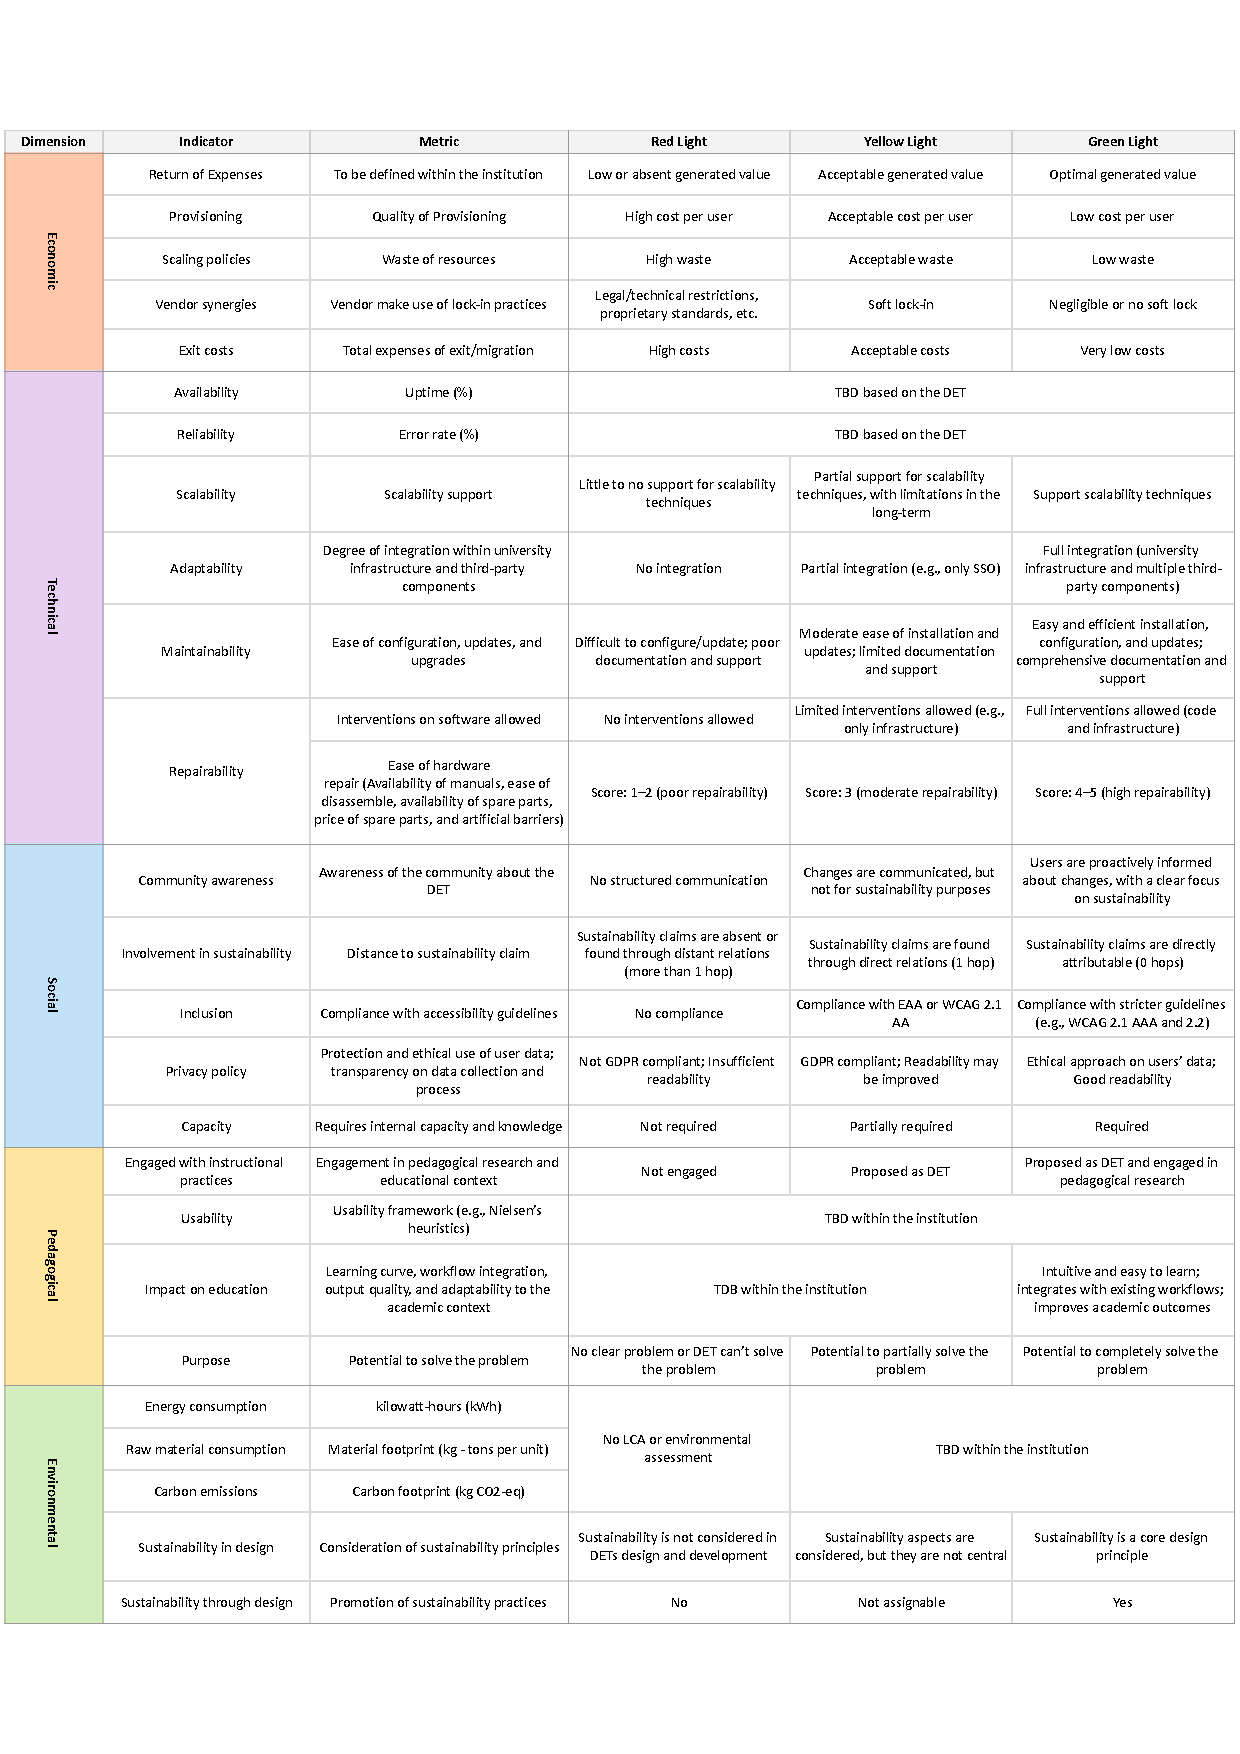
\includegraphics[width=1\linewidth]{attachments/indicators_overview.pdf}
    \caption{Overview of indicators}
    \label{fig:A1_attach_indicators_overview}
\end{figure}

\begin{figure}[ht]
    \centering
    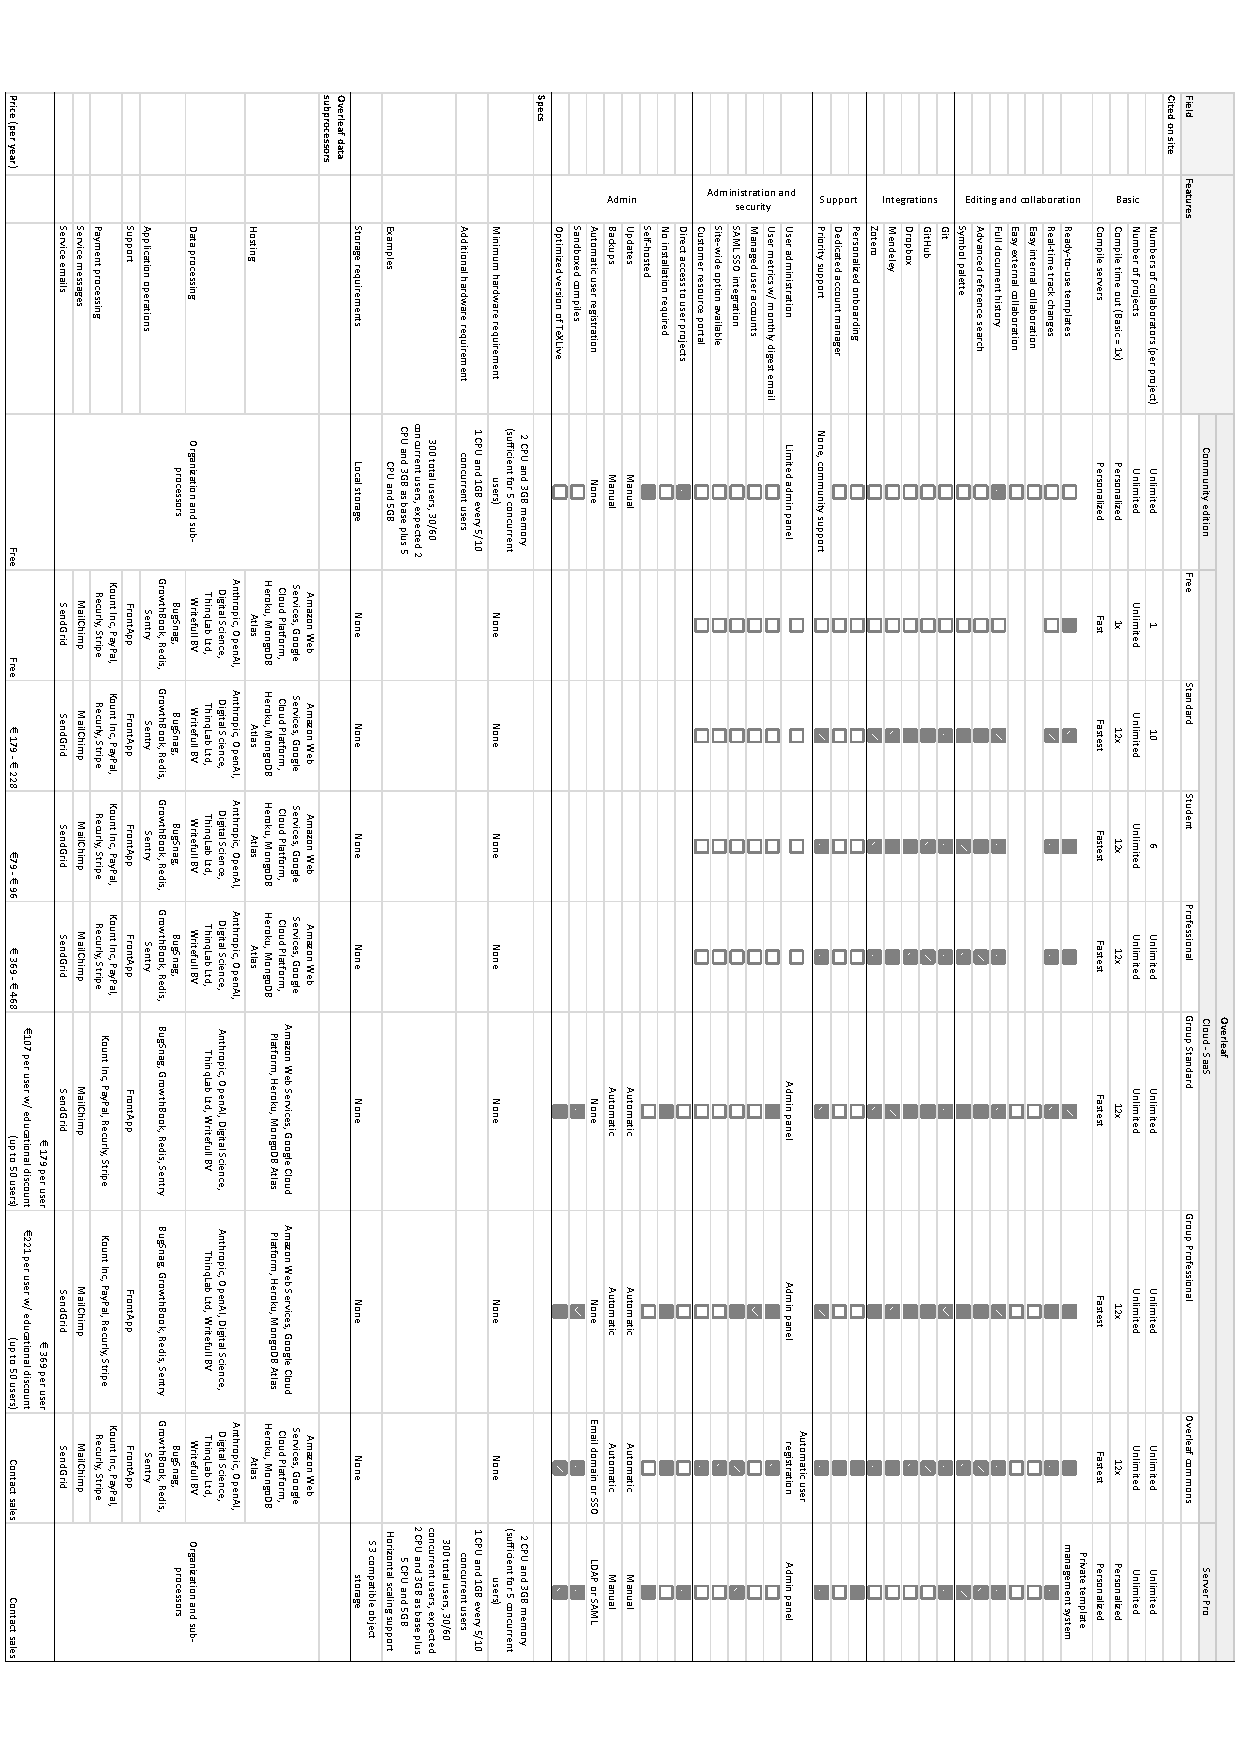
\includegraphics[width=1\linewidth]{attachments/overleaf_overview.pdf}
    \caption{Comparison between Overleaf versions}
    \label{fig:A2_attach_overleaf_overview}
\end{figure}

\newpage






\end{document}
